%% FEUP THESIS STYLE for LaTeX2e
%% how to use feupteses (portuguese version)
%%
%% FEUP, JCL & JCF, 31 Jul 2012
%%
%% PLEASE send improvements to jlopes at fe.up.pt and to jcf at fe.up.pt
%%
%% Example for PDI course
%%

%%========================================
%% Commands: pdflatex tese
%%           bibtex tese
%%           makeindex tese (only if creating an index) 
%%           pdflatex tese
%% Alternative:
%%          latexmk -pdf tese.tex
%%========================================

\documentclass[11pt,a4paper,twoside,openright]{report}

%se quiser tirar espaço em branco entre capitulos, adcionar openany no documentclass
%% For iso-8859-1 (latin1), comment next line and uncomment the second line
\usepackage[utf8]{inputenc}

%serve para esconder titulo do capitulo
%\usepackage{titlesec}
%\titleformat{\chapter}[display]
%{\normalfont\bfseries}{}{0pt}{\Huge}

%\usepackage[latin1]{inputenc}

%% Portuguese version

%% MIEEC options
\usepackage[portugues,mieec]{feupteses}
\usepackage{enumitem}

%\usepackage[portugues,mieec,juri]{feupteses}
%\usepackage[portugues,mieec,final]{feupteses}
%\usepackage[portugues,mieec,final,onpaper]{feupteses}

%% For other degrees
%\usepackage[portugues]{feupteses} % you must define the degree bellow

%% Options: 
%% - portugues: titles, etc in portuguese
%% - onpaper: links are not shown (for paper versions)
%% - backrefs: include back references from bibliography to citation place

%% Uncomment to create an index (at the end of the document)
%\makeindex

%% Path to the figures directory
%% TIP: use folder ``figures'' to keep all your figures
\usepackage{graphics}
\usepackage{subfig}
\usepackage[section]{placeins}
\usepackage{float}
\usepackage{tikz}
\usepackage{notoccite}
\usepackage{amssymb}
\usepackage{pgfgantt}
\usetikzlibrary{shapes.geometric}
\usetikzlibrary{shapes.arrows}
\usepackage{multirow}
\usepackage{colortbl} 


\graphicspath{{figures/}}

%%----------------------------------------
%% TIP: if you want to define more macros, use an external file to keep them
%some macro definitions

% format
\newcommand{\class}[1]{{\normalfont\slshape #1\/}}

% entities
\newcommand{\Feup}{Faculdade de Engenharia da Universidade do Porto}

\newcommand{\svg}{\class{SVG}}
\newcommand{\scada}{\class{SCADA}}
\newcommand{\scadadms}{\class{SCADA/DMS}}

%%----------------------------------------

%%========================================
%% Start of document
%%========================================
\begin{document}
	
	%%----------------------------------------
	%% Information about the work
	%%----------------------------------------
	\title{Odometria visual em robôs para a agricultura
		com câmara(s) com lentes olho de peixe}
	\author{Sérgio Miguel Vieira Pinto}
	
%	\degree{\textsc{Relatório de Progresso}}
	%% Uncomment next line for date of submission
	%\thesisdate{31 de Julho de 2008}
	
	%% Comment next line for copyright text if not used
	\copyrightnotice{Sérgio Pinto, 2018}
	
	\supervisor{Orientador}{Prof. Dr. Armando Jorge Sousa}
	\supervisor{Coorientador}{Prof. Dr. Filipe Neves dos Santos}
	
	
	%% Uncomment committee stuff in the final version if used
	%\committeetext{Aprovado em provas públicas pelo Júri:}
	%\committeemember{Presidente}{Nome do presidente do júri}
	%\committeemember{Arguente}{Nome do arguente do júri}
	%\committeemember{Vogal}{Nome do vogal do júri}
	%\signature
	
	%% Specify cover logo (in folder ``figures'')
	\logo{uporto-feup.pdf}
	
	%% Uncomment next line for additional text  below the author's name (front page)
	\additionalfronttext{Versão de Trabalho}
	\setcounter{tocdepth}{3}
	%%----------------------------------------
	%% Preliminary materials
	%%----------------------------------------
	
	% remove unnecessary \include{} commands
	
	\begin{Prolog}
		%\chapter*{Resumo}



O desenvolvimento da robótica tende a ser cada vez mais significativo no meio agrícola, nomeadamente no contexto de vinha de encosta. Contudo, este contexto pode não ser facilitador uma vez à localização no mesmo se baseia em sistemas de odometria das rodas e/ou de posicionamento global por satélites estes sistemas tendem a falhar devido às encostas  e inclinações do terreno, afetando a qualidade do sinal de satélite e precisão da odometria das rodas.

Recorrendo-se a  tecnologias complementares é possível melhorar a precisão e auxiliar os algoritmos de localização. O robô Agrob incorporado no projeto ROMOVI e desenvolvido no INESTEC  utiliza câmaras para o tratamento e manutenção das videiras, podendo estas auxiliar na localização, através de Odometria Visual. O uso da lente olho de peixe aumenta o campo de visão reforçando a estabilidade do sistema com maior captura de pontos característicos.

Através da captura e processamento de imagens é estimado o deslocamento entre imagens que num fluxo de imagens resulta numa localização do robô. Desta forma, nesta dissertação é desenvolvido um algoritmo de análise de imagens com objetivo de obter a translação e rotação entre imagens que concatenadas originam a localização do robô.


Na presente dissertação foram realizados vários testes, tais como, estático, movimento linear, rotação angular, movimento semi-quadrangular e movimento quadrangular, de forma a verificar a robustez do algoritmo.


Esta dissertação apresenta um algoritmo de localização desenvolvido em ROS e com câmara com lente olho de peixe. Os testes realizados são ilustrados graficamente e comparados com a Odometria das rodas do robô.


\chapter*{Abstract}


The development of robotics tends to be increasingly significant in the agricultural environment, particularly in the context of hillside vineyards. However, in this context may not be easy since the localization it is based on global positioning systems by wheels' odometry and / or satellites. These systems tend to fail due to terrain slopes and slopes, affecting the quality of the satellite signal and the accuracy of the wheels' odometry.


Using complementary technologies it is possible to improve accuracy and auxiliary localization algorithms. The Agrob robot incorporated in the ROMOVI project and developed in INESTEC uses cameras for the treatment and maintenance of the vines, these can auxiliary the localization through Visual Odometry.  The use of the fisheye lens increases the field of vision reinforcing the stability of the system with greater capture of characteristic points.

Through the capture and processing of images are estimated the displacement between images, which in a flow of images results in a robot localization. In this way, is developed an algorithm to analyze the images and obtain the translation and rotation matrix between images that through a matrix concatenation is obtained the robot localization.

In the present dissertation several tests were performed, such as, static, linear movement, angular rotation, semi-quadrangular movement and quadrangular movement in order to verify the robustness of the algorithm.


This dissertation presents a localization algorithm developed in ROS and with a camera with a fisheye lens. The tests performed are ilustrated graphically  and compared with the wheels' Odometry of robot.
		\tableofcontents
		\listoffigures
		\listoftables
		\chapter*{Abreviaturas e Símbolos}
%\addcontentsline{toc}{chapter}{Abbreviations}
\chaptermark{ABREVIATURAS E SÍMBOLOS}

\begin{flushleft}
\begin{tabular}{l p{0.8\linewidth}}
INESC-TEC & Institute for Systems and Computer\\ Engineering, Technology and Science \\
GPS & Global Position System\\
GNSS & global Navigations Satellite System \\
INS &  Inertial Navigation System\\
OV & Odometria Visual\\
UAV & Unmanned aerial vehicle \\
NASA & National Aeronautics and Space Administration\\
RANSAC & RANdom SAmple Consensus\\
FAST & Feature from Accelerated Segment Test\\
SIFT & Scale Invariant Feature Transform\\
DoG & Diference of Gaussians\\
SURF & Speeded Up Robust Features\\
ORB & Oriented FAST and Rotation-Aware BRIEF\\
BRIEF & Binary Robust Independent Elementary Features\\
SVD & Singular Value Decomposition\\
FLIR & Foreard Looking Infra-Red\\
ROS & Robot Operating System \\
IDE & Integrated Development Environment 
\end{tabular}
\end{flushleft}

  % the list of abbreviations used
	\end{Prolog}
	
	%%----------------------------------------
	%% Body
	%%----------------------------------------
	
	\StartBody
	
	%% TIP: use a separate file for each chapter
	% !TeX spellcheck = <none>
\chapter{Introdução} \label{chap:introdução}
Este capítulo levanta algumas questões a serem respondidas durante a dissertação e fornece uma  visualização dos objetivos e alcance do documento.
 
\section{Enquadramento} \label{sec:enquadramento}
A necessidade de uma maior eficiência nos trabalhos do quotidiano, levou a um desenvolvimento da robótica, tornando os robôs mais autónomos e eficazes. Com o avanço da robótica é possível aumentar o número de horas de trabalho sem perdas de eficiência e desgaste que um ser humano teria, obtendo uma diminuição de custos.

Em Portugal a vinicultura tem vindo a ter um crescimento constante e com ela um aumento da necessidade da robótica. A monitorização das vinhas é essencial para qualidade do produto final , sendo esta, muitas vezes difícil de se realizar com eficácia. Assim , através da robótica essa eficácia pode ser conseguida, realizando trabalhos de maior dificuldade para o Homem a um custo mais reduzido, tal como a monitorização dia e noite, 24h por dia , dos terrenos. 

Desta forma, o projeto \textit{RoMoVi}, desenvolvido pelo centro de Robótica do INESC-TEC, pretende desenvolver um robô, no âmbito da robótica para a agricultura, capaz de podar, monitorizar e fertilizar as encostas de vinhas inclinadas \cite{Mendes2016}. Este projeto tem disponíveis três plataformas : o \textit{AGROB V16}, \textit{AGROB V15}, \textit{AGROB V14}, sendo a presente dissertação desenvolvida no contexto do projeto \textit{RoMoVi} e linha de investigação apelidada de \textit{AGROB} \cite{RN32}.

Neste projeto é necessário a implementação de uma sistema de localização que seja de baixo custo e adequado à aplicação em contexto de vinha de encosta.

A precisão na localização de robôs é fundamental para a sua eficácia e funcionamento. Existem vários tipos de localizações , tais como \textit{Global Position System} (GPS), \textit{Global Navigations Satellite System} (GNSS), \textit{Inertial Navigation System} (INS), Odometria através das rodas, laser/ultrasonico Odometria e Odometria Visual (OV). Contudo, cada tecnologia tem as suas fraquezas. Odometria das rodas é uma tecnologia simples para estimação da posição mas a inclinação do terreno e deslizamento das rodas no pavimento causa erros grandes. Laser/ultrassónico  Odometria utiliza energia acústica para detetar objetos e medir distâncias entre os sensores e os objetos, contudo estes sensores são muito sensiveis ao ruido . INS é ótimo para a acumulação de deslizamento e têm grande precisão, mas em contrapartida é muito dispendiosa a nível monetário e não é a ideal para soluções comerciais. Apesar de a GPS  ser a solução mais comum para localização absoluta por causa da não acumulação de erro, não é útil para este projeto devido ao fraco sinal dos satélites. Tal, deve-se à inclinação dos terrenos e possibilidades de céu nublado. Para além disso, a utilização de GPS este também se torna cara para a precisão em centímetros. \cite{Aqel2016}

Por último, OV é uma tecnologia que envolve um fluxo de imagens adquiridas através de uma câmara e posteriormente analisadas permitindo obter a estimação da localização. É um método barato e com grande precisão, que se enquadra neste projeto. As desvantagens desta localização passam pela necessidade de um bom processamento e a possibilidade de existência de erros causados por objetos dinâmicos e/ou sombras.

\section{Motivação e Objetivos} \label{sec:context}

Com as dificuldades de localização já mencionadas no capitulo anterior, a tecnologia mais indicada é a Odometria Visual (OV). Esta será implementada num raspberry pi com uma câmara com lente olho de peixe para obter maiores ângulos de captura.

Assim, utilizando a câmara com lente de olho de peixe com um ângulo de cerca de 180º é possível capturar um fluxo de imagens com imensa informação. Informação essa que será analisada por um algoritmo implementado num raspberri pi, da qual resultará uma estimativa de localização.

A utilização de visão será sensível às condições de iluminação e reflexões. Com isto, o processamento de imagem terá de ser rigoroso para que o erros sejam mínimos.

Na presente dissertação pretende-se desenvolver um sistema de auxílio à localização que seja de baixo custo e adequado à aplicação em contexto de vinha de encosta. Neste sentido será utilizada a OV na qual resultará um avaliação da precisão do método.

	%\chapter{Trabalho} \label{chap:sota}
\section{Interações com orientador}\label{chap:descricao}
Na fase Reordenação de Escolhas pelo Estudante, a 5 de Outubro, esclareci alguma dúvidas por email com o professor Armando Sousa sobre o tema da dissertação.
		
A primeira reunião, a 6 de Novembro, serviu para esclarecer quais os objetivos da dissertação e para o Orientador recomendar alguns temas a serem estudados pelo estudante, mais especificamente, estudo do \textit{ROS}, leitura de alguns documentos sobre trabalhos realizados no projeto \textit{RoMoVi}, contextualização com odometria visual e processamento/análise de imagens.

A 13 de Novembro realizou-se outra reunião para esclarecimento de dúvidas sobre os tópicos: utilizar imagem mono ou stereo , especificações necessárias na lente olho de peixe, \textit{ROS}.

Por ultimo existiu contacto por email, para receber feedback acerca deste documento.
	

\section{Trabalho realizado}\label{sec:proximas etapas}

Inicialmente foi feita uma leitura de todos os documentos aconselhados pelo Orientador. Desta forma foram surgindo duvidas das quais resultaram pesquisas na internet e outras foram esclarecidas pelo Orientador. Mais tarde foi realizado um estudo geral do mercado e quais os componentes necessário a utilizar na dissertação.

Em paralelo foi inicializada a contextualização com o \textit{ROS}, realizando a sua instalação e primeiros tutoriais.

	\chapter{Revisão Bibliográfica}\label{chap:odometria visual}


Odometria Visual (OV) é um método de estimação da posição através de um fluxo de imagens de uma câmara (Sistema monocular) ou várias câmaras (Sistema estéreo) \cite{Ericson2018}. OV foi durante muitos anos, um dos estudos pioneiros de Nister, Narodistsky and Bergen \cite{Nisterb}. O trabalho deles resultou num algoritmo em que extrai pontos característicos de  uma imagem, cruzavam com outros e , no fim, usavam para obter uma estimativa de movimento. 

A implementação de OV em locais interiores é bem sucedida enquanto que em locais exteriores são notórios alguns problemas. Alguns fatores, como sombras e objetos dinâmicos, causam  dificuldades de localização em locais exteriores. Para OV funcionar eficientemente é necessário iluminação suficiente e ambiente estático para permitir que o movimento seja extraído corretamente. 

OV tem uma ampla aplicação e foi implementada em diferentes campos eficientemente. Os domínios de aplicação incluem robótica e automação. Os tipos de aplicação são sistemas robóticos móveis, tais como terrestre, subaquáticos, aéreos e espaciais.

Em termos terrestres, a OV é usada para a navegação e deteção de objetos eficientemente. Quanto aos sistemas robóticos moveis subaquáticos, a OV tem um papel significativo nos veículos autónomos subaquáticos e sistemas de inspeção de recifes de corais \cite{Aqel2016}. A nível aéreo, a OV é aplicada a \textit{drones} (UAVs) para melhorar a performance de navegação autónoma. Por último, na exploração espacial , a OV é usada para estimar o movimento do robô NASA Mars  \cite{Cheng} .


Na indústria , OV desempenha um papel importante. É aplicada em sistemas de apoio à condução, tal como em sistema de travagem assistida baseados em visão.  Em grande parte dos veículos são utilizados sensores de visão para navegação e deteção de obstáculos devido ao sinal de GPS ser fraco, ser de leve implementação (em veículos pequenos é crucial) e ser suficientemente eficaz para o baixo custo.  Na agricultura é utilizada OV para estimação relativa em relação às culturas \cite{ericson2008visual,Mendes2016}.


\section{Contextualização}

Nesta secção é feito um breve resumo da computação em sistemas de OV.

Com base no artigo \cite{VOpart1}, um determinado agente ligado a um sistema de câmaras move-se num determinado ambiente e captura imagens em instantes de tempo discreto \textit{k}. Caso o sistema seja composto por visão monocular, o conjunto de imagens capturadas em intervalos de \textit{k} é representado por  \textit{$I_{0:n}$}  = \{\textit{$I_0$}, ..., \textit{$I_n$}\}. 
No caso de ter visão estéreo, então existem duas imagens (esquerda e direita) em cada instante de tempo, representadas por \textit{$I_{e,0:n}$} = \{\textit{$I_{e,0}$}, ..., \textit{$I_{e,n}$}\} e \textit{$I_{d,0:n}$} = \{\textit{$I_{d,0}$}, ..., \textit{$I_{d,n}$}\}. 
Na Figura ~\ref{fig:arch} é apresentado uma ilustração deste cenário. 


\begin{figure}[h!] %colocar figura a seguir ao texto anterior
	\begin{center}
		\leavevmode		
		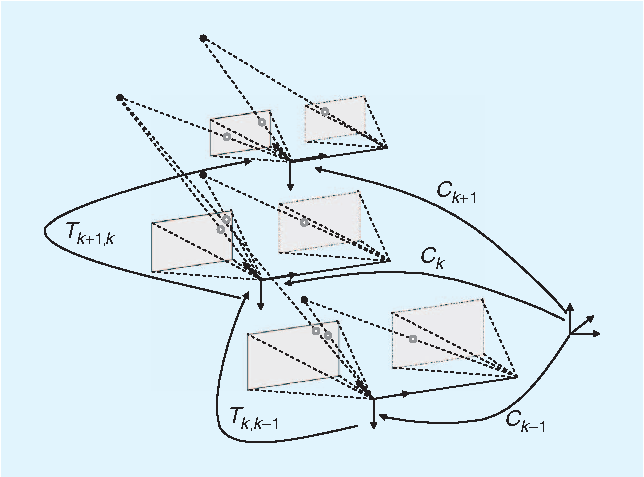
\includegraphics[width=0.65\textwidth]{problVO}
		\caption{Ilustração do problema de OV para visão estéreo.  \cite{VOpart1}}
		\label{fig:arch}
	\end{center}
\end{figure}

Por simplificação, é assumido que o sistema de coordenadas da câmara coincide com o sistema de coordenadas do agente. No caso de sistema estéreo, considera-se que o sistema de coordenadas da câmara esquerda pode ser utilizado como origem sem perda de aspetos gerais.

As posições de uma câmara em instantes de tempo adjacentes \textit{k-1} e \textit{k} estão relacionadas por uma transformação de corpo rígido $T_{k,k-1}$ $\in\ $ $R^{4x4}$ da seguinte forma: \[ T_{k,k-1} = \left[\begin{array}{cc} R_{k,k-1} & t_{k,k-1} \\  0 & 1 \\ \end{array} \right] \]
onde $R_{k,k-1}$ $\in$ $R^{3x3}$ é a matriz de rotação e $t_{k,k-1}$ $\in$ $R^{3x1}$ é o vetor de translação. O conjunto $T_{1:n}$ = \{ $T_{1,0}$, ..., $T_{n,n-1}$ \} contém todos os movimentos sequenciais da câmara. Para simplificar
a notação, a partir de agora, $T_k$ será usado em vez de $T_{k,k-1}$. Finalmente, o conjunto das posições da câmara $C_{0:n}$ = \{ $C_0$, ..., $C_n$ \} contém as transformações da câmara em relação à coordenada da frame inicial no instante \textit{k} = 0. A posição atual $C_n$ pode ser calculada juntando todas a transformações $T_k$ ( \textit{k} = 1 ... n\ ), e assim, $C_n$ = $C_{n-1}T_n$, com $C_0$ sendo a posição da câmara no instante \textit{k} = 0, que pode ser definida arbitrariamente pelo utilizador.

A principal tarefa em um sistema OV é calcular a transformação relativa $T_k$ a partir das imagens $I_k$ e $I_{k-1}$, e depois juntar as transformações para recuperar a trajetória completa $C_{0:n}$ da câmara. Isto significa que o sistema consegue recuperar de forma incremental a trajetória, posição após posição.

A fim de efetuar um sistema de OV é necessário realizar várias etapas. A Figura ~\ref{fig:etapVO} ilustra um diagrama de blocos com a metodologia a utilizar.

\begin{figure}[h!] %colocar figura a seguir ao texto anterior
	\begin{center}
		\leavevmode		
		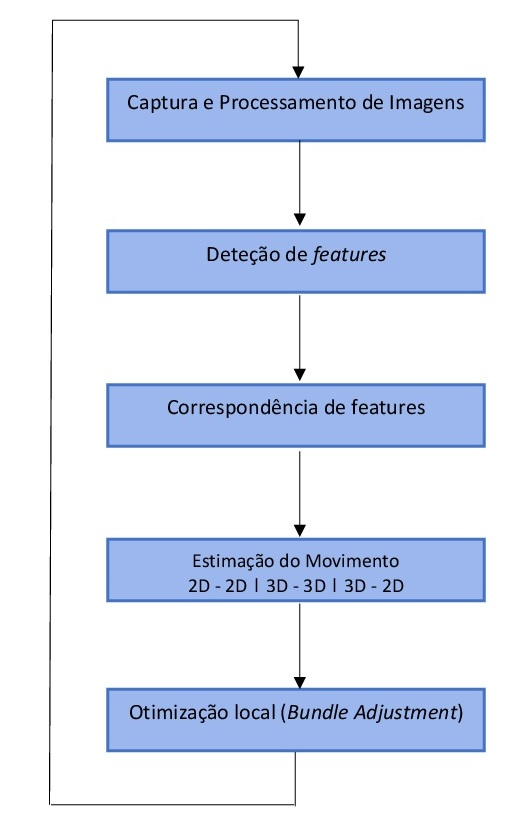
\includegraphics[width=0.4\textwidth]{etapVO}
		\caption{Etapas de um sistema de Odometria Visual.}
		\label{fig:etapVO}
	\end{center}
\end{figure}

Desta forma, a primeira etapa ilustra o processo de captura de uma nova imagem \textit{$I_k$}, ou um par de imagens no caso de um sistema estéreo. Nesta mesma etapa é necessário o processamento da imagem para remover possíveis deformações das imagens ou efeitos de lentes.

A segunda etapa apresenta dois métodos diferentes para encontrar características \footnote{é uma região na imagem que difere da sua vizinhança em termos de intensidade, cor e textura.}, que consistem na procura de características visuais salientes que possam corresponder noutras imagens.

A terceira etapa apresenta dois métodos diferentes para correlacionar características. Nesta mesma etapa são aplicados algoritmos de correção  para remover eventuais erros de correspondência. Uma solução para o problema é a utilização do algoritmo RANSAC.

A quarta etapa consiste no cálculo do movimento relativo $T_k$ entre os instantes de tempo \textit{k} - 1 e \textit{k}. Após a obtenção do $T_k$ então é possível calcular a posição da câmara $C_k$ por junção do $T_k$ com a posição anterior $C_{k-1}$.

Finalmente, a última etapa descreve a aplicação do algoritmo de otimização local, \textit{Buldle Adjustment} , ao longo das últimas características com o objetivo de obter uma estimativa mais precisa da trajetória local.


\section{Parâmetros Intrínsecos} \label{section:Intrin}

A formação de uma imagem em uma câmara ocorre com a entrada de feixes de luz através de uma abertura na câmara e a projeção desses feixes em uma tela, também chamada de plano de imagem.

Em uma câmara real, um ponto no mundo reflete diversos feixes de luz. Se todos os feixes refletidos por esse ponto convergirem para um mesmo ponto no plano de imagem, então é dito que a imagem está focada. O modelo de projeção perspetiva é uma simplificação da câmara real.

O modelo de projeção perspetiva é apresentado na Figura ~\ref{fig:modelcamera}. O centro de projecção \textbf{O} é a origem do sistema de coordenadas da câmara e também o centro da câmara. O eixo-z do sistema de coordenadas da câmara é chamado eixo-principal. O plano \textit{z} = \textit{f} é o plano de imagem e a intersecção do plano de imagem com o eixo-principal é chamado ponto principal. Considere $\textbf{X} = [X,Y,Z]^T$ as coordenadas de um ponto no mundo referentes ao sistema de coordenadas da câmara. A intersecção do plano de imagem com o segmento de reta ligando \textbf{X} e \textbf{O} é a projeção de \textbf{X} e é referenciada como \textbf{x}. Por semelhança de triângulos observa-se que \textbf{x} = $[\textit{f} \frac{X}{Z} , \textit{f} \frac{Y}{Z} , \textit{f}]$ em relação à câmara. Como a última coordenada de \textbf{x} será sempre \textit{f}, ela será desconsiderada nas equações daqui em diante.

\begin{figure}[h!]  %colocar figura a seguir ao texto anterior
	\centering
	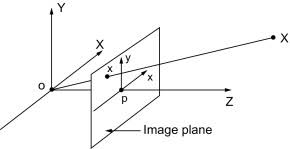
\includegraphics[width=0.6\linewidth]{figures/pinholemodel} 
	\caption{Esquema do modelo de projeção perspetiva. \cite{Yousif2015}}
	\label{fig:modelcamera}  %30 years. Figure 3 a)
\end{figure}

Assim, o mapeamento do mundo 3-D para uma imagem 2-D é obtido através da equação de projeção perspetiva :
\[  \textbf{$\lambda$} \left[ \begin{array}{c} u\\v\\1\\ \end{array} \right] = 
KX = \left[ \begin{array}{ccc} \alpha_u  & 0 & \textit{u}_0 \\ 
0 & \alpha_v & \textit{v}_0 \\ 
0 & 0 & 1 \\
\end{array} \right] \left[ \begin{array}{c} X \\ 
Y \\ 
Z \\ 
\end{array} \right] , \]
onde $\lambda$ é o facto de profundidade, $\alpha_u$ e $\alpha_v$ são as distâncias focais, e $\textit{u}_0$ e $\textit{v}_0$ são as coordenadas centrais da projeção da imagem. Estes parâmetros são conhecidos como parâmetros intrínsecos que dependem de câmara para câmara. Quando o campo de visão da câmara é superior a 45º , os efeitos da distorção radial são visíveis e causam erros superiores.

Note que a última coordenada \textit{w} é a escala da coordenada homogénea e não a distância focal f, que como já foi dito, é desconsiderada daqui em diante. Daqui em diante as coordenadas homogéneas serão representadas por \textbf{x} e \textbf{X} 


\subsection{Lente olho de peixe}

Em câmaras com lentes olho de peixe os parâmetros intrínsecos são diferentes. Estes tipos de lentes são similares à visão humana, onde a imagem resultante tem grande resolução central e baixa resolução nos pontos mais distantes do centro. O modelo mais comum de lentes olho de peixe é o modelo equiangular ,  \[ r = k \theta ,  \] onde k é uma constante \cite{Hansen2009}.

\begin{figure}[h!] %colocar figura a seguir ao texto anterior
	\begin{center}
		\leavevmode		
		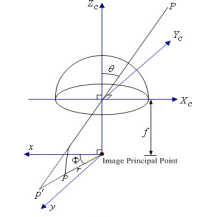
\includegraphics[width=0.4\textwidth]{fisheyemodel}
		\caption{Projeção de um ponto no mundo no plano de imagem. Onde o ponto p' representa projeção perspetiva e o ponto p com o modelo equiangular com distorção da lente olho de peixe. \cite{Srestasathiern2014,Kannala2004}}
		\label{fig:fishvspinhole} 
	\end{center}
\end{figure}

A Figura ~\ref{fig:fishvspinhole} representa a diferença entre a representação de um ponto \textit{P} na imagem captura . Desta forma, o ponto \textit{p'} usa o modelo da projeção perspetiva e o ponto \textit{p} o modelo equiangular onde se visualiza a distorção da lente olho de peixe.

Assim, o algoritmo é descrito pela Figura ~\ref{fig:fisheyealgortim}

\begin{figure}[h!]
	\centering
	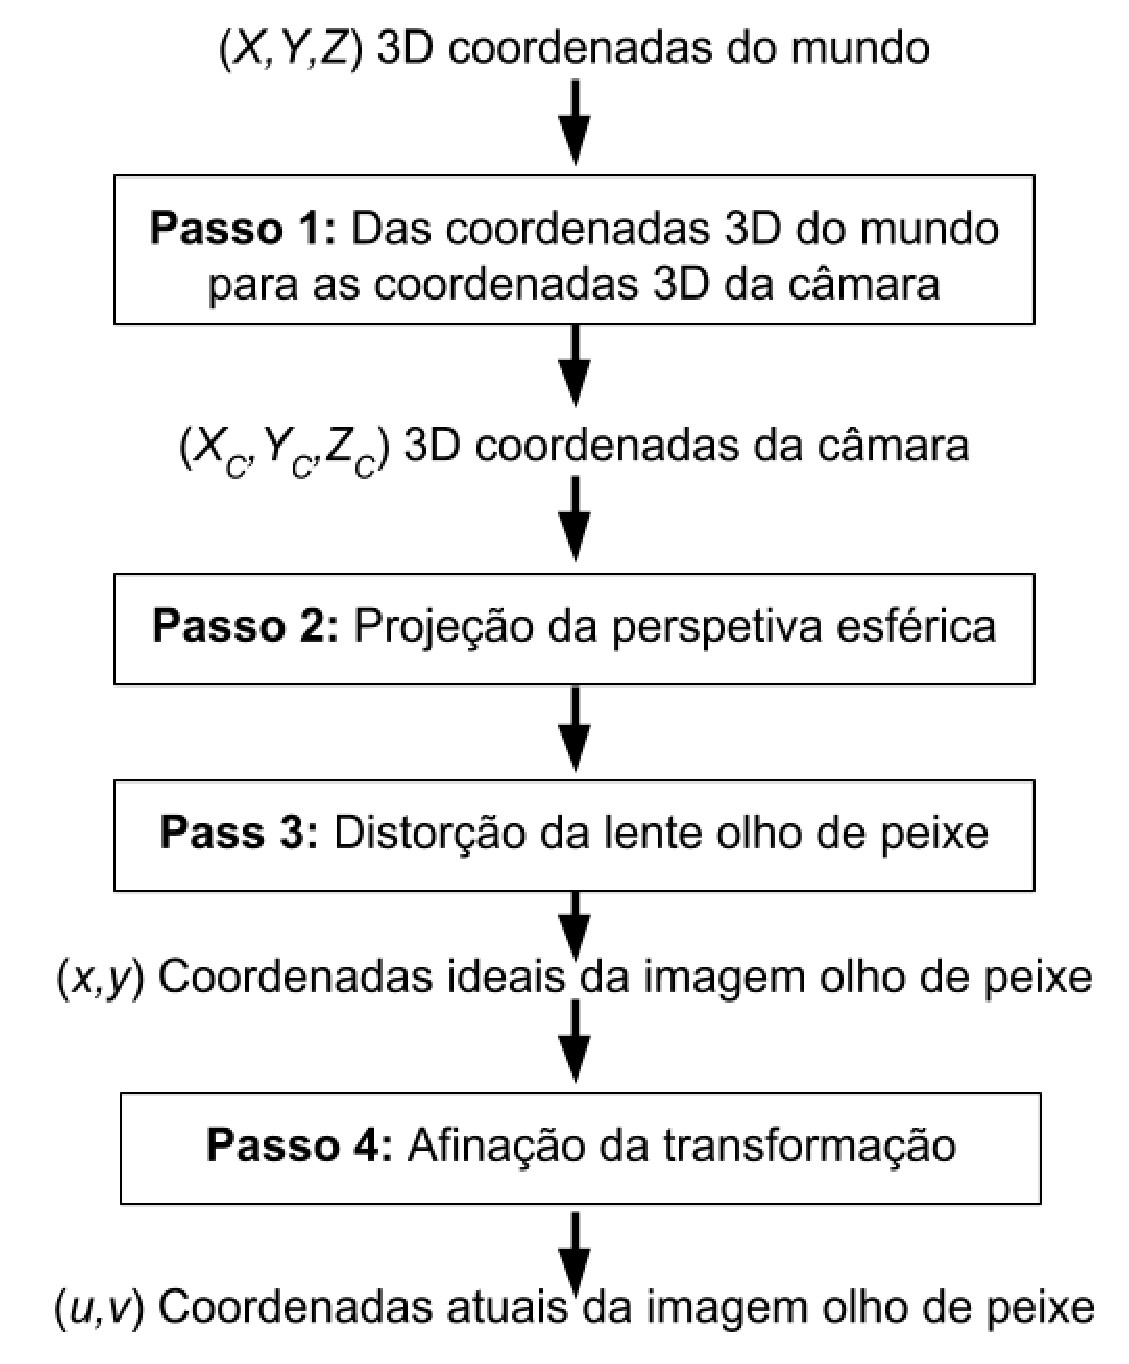
\includegraphics[width=0.4\linewidth]{figures/fisheyealgortimpt}
	\caption{Algoritmo de construção da imagem com lente olho de peixe. \cite{Ying2006}}
	\label{fig:fisheyealgortim}
\end{figure}

Passo 1:  \[ \textbf{P}_\textbf{C} = \textbf{R}\textbf{P}_\textbf{W} + \textbf{t} , \] onde $\textbf{P}_\textbf{C}$ é o ponto capturado na imagem, $\textbf{P}_\textbf{W}$ é o ponto no mundo, \textbf{R} é a matriz de orientação e \textbf{t} é o vetor da posição. Os parâmetros \textbf{R} e \textbf{t} são parâmetros extrínsecos. 

Passo 2: O ponto $\textbf{P}_\textbf{C}$ é projetado com perspetiva de uma esfera resultando o ponto \textbf{p} \[ \textbf{p = $\frac{\textbf{P}_\textbf{C}}{ \| \textbf{P}_\textbf{C} \| }$ } = ( sin \phi cos \theta, sin \phi sin \theta, cos \phi)^T  . \]

Passo 3: O ponto \textbf{p} é mapeado para m no plano de imagem com distorção da lente da câmara \[ m = D(p) , \] onde m = (x,y) e D é o modelo de distorção da lente olho de peixe. 

Passo 4: O ponto m é transformado em m' usando a transformação de afinidade: \[ m' = K_A(m) , \] onde m' = (u,v). A imagem obtida é a imagem atual da câmara com lente olho de peixe que é igual : \[ \widetilde{m}'\ ' = K_A \widetilde{m}'\  ,\] onde $\widetilde{m}'\ $ = $(x,y,1)^T$ e $\widetilde{m}'\ '$ = $(u,v,1)^T$ e $K_A$ =$\left[ \begin{array}{ccc}
r & s & u_0 \\ 
0 & 1 & v_0 \\ 
0 & 0 & 1
\end{array} \right]$ 


Desta forma, concluímos que existem 12 parâmetros para as lentes olho de peixe: 4 parâmetros de transformação de afinidade, 4 radiais e 4 parâmetros de distorção tangencial. Estes parâmetros são os parâmetros intrínsecos das lentes olho de peixe.




\section{Parâmetros Extrínsecos}

Em geral os pontos do mundo são descritos em relação a um sistema de coordenadas global. A relação entre os dois sistemas é dada por uma transformação de corpo rígido do tipo

\[ \textbf{X} = \textbf{R}\textbf{X}_\textbf{W} + \textbf{T},  \]

onde $\textbf{X}_\textbf{W}$ são as coordenadas do ponto \textbf{X} em relação ao sistema de coordenadas global. A matriz \textit{R} $\in$ \textit{$SO(3)$} é a rotação que alinha o sistema de coordenadas global com o sistema de coordenadas da câmara e $\textbf{T}$ $\in$ $\mathbf{R^3}$ é o vetor de translação entre os dois sistemas de coordenadas. Os parâmetros de \textit{R} e \textbf{T} são chamados de parâmetros extrínsecos e a matriz 

\[ [\textit{R}|\textbf{T}] = \left[ \begin{array}{cccc}
r_{11} & r_{12} & r_{13} & t_1 \\ 
r_{21} & r_{22} & r_{23} & t_2 \\ 
r_{31} & r_{32} & r_{33} & t_3
\end{array} \right] \]

é a matriz de parâmetros extrínsecos. A Figura ~\ref{fig:parExt} mostra a relação entre os dois sistemas de coordenadas.

\begin{figure}[h!]
	\centering
	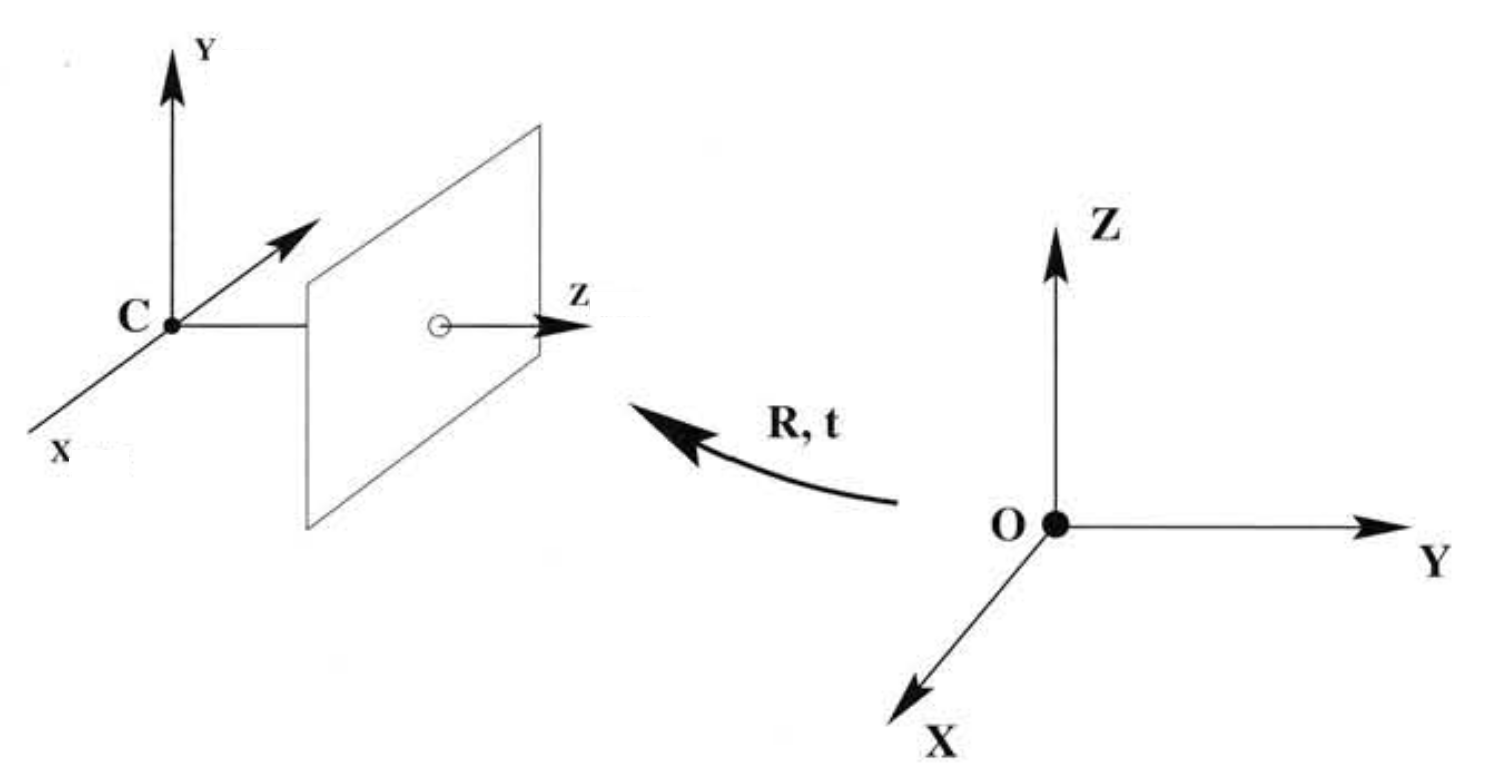
\includegraphics[width=0.7\linewidth]{figures/parExt}
	\caption{Parâmetros que definem a posição e orientação do sistema de coordenadas da câmara com um sistema de coordenadas global.}
	\label{fig:parExt}
\end{figure}


\section{Detetores de Características}\label{detCar}

A deteção de características é o processo responsável por determinar características numa imagem. Uma característica pode ser uma região de uma cor específica, um determinado padrão na imagem, um ponto onde ocorre a variação de cores ou outra informação que possa ser extraída da imagem. Estas características devem ser escolhidas de forma a serem possíveis de encontrar e recuperar futuramente. 

Relativamente a sistemas de OV, foi descoberto que a distribuição de características numa imagem afeta de uma forma considerável os resultados obtidos. Em particular, quanto mais características encontradas mais estáveis são os resultados da estimação do movimento, mas o tempo de processamento é maior e pode causar perdas de \textit{frames} importantes. As características são procuradas numa imagem através de um detetor de características. Para ser um bom detetor de características têm de obedecer às seguintes características \cite{Fraundorfer2012}:
\begin{itemize}
	\item Precisão na localização, tanto em posição como em escala.
	\item Repetibilidade, garante que uma grande percentagem das caracteristicas visíveis a duas imagens serão identificadas em ambas as imagens.
	\item Eficiência computacional, está relacionada ao tempo que o algoritmo de deteção necessita para identificar as características de uma imagem.
	\item Robustez ao ruído e desfocagem
	\item Distinção , de modo que as características possam ser correspondidas precisamente entre imagens diferentes.
	\item Invariância à iluminação e mudanças geométricas, garante que a característica será identificada igualmente com ou sem a transformação.
\end{itemize}

Na área de OV os detetores de características, tais como \textit{cantos}\footnote{é definido como um ponto de intersecção de duas ou mais arestas.} ou \textit{blobs}\footnote{são regiões mais brilhantes (ou mais escuras) do que o meio circundante.}, são muito importantes porque é possível saber com precisão a sua posição numa imagem. 

Entre estes dois tipos de detetores, os detetores de canto são computacionalmente mais rápidos mas menos distintos. Adicionalmente, detetores de canto estão melhores localizados em posições de imagens mas são menos localizados em escala. Isto significa que os detetores de canto podem não ser tão bem detetados que os detetores de \textit{blob} quando existem grandes variações de escala e pontos visíveis. Contudo, detetores de \textit{blob} não são bons em certos ambientes \cite{Fraundorfer2012}.

\subsection{Detetores de Cantos}

Um canto em uma imagem é o ponto onde há uma grande variação de intensidade dos \textit{pixels} em duas direções dominantes. 

\subsubsection{Harris}

O detetor de cantos Harris é um dos métodos mais recentes (1988). A ideia base no algoritmo de Harris é analisar um ponto através das características e de uma pequena vizinhança. Através da alteração da janela em várias direções do ponto , a média da intensidade da janela deve alterar significativamente se o ponto for um canto. Os cenários possíveis são ilustrados na Figura ~\ref{fig:harriscornerdetection}

\begin{figure}[h!]
	\centering
	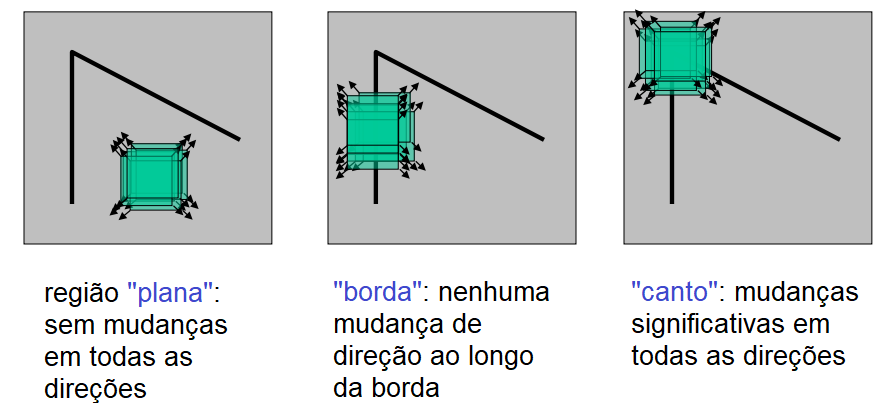
\includegraphics[width=0.7\linewidth]{figures/HarrisCornerDetection}
	\caption{Detetor de cantos Harris. \cite{VisualOdometryRodasVehicles}}
	\label{fig:harriscornerdetection}
\end{figure}

Desde que a janela seja alterada em várias direções , o algoritmo deve obter o mesmo resultado mesmo que a imagem tenha sofrido uma rotação. O mesmo não acontece caso a imagem sofra um zoom , o algoritmo não fornece os mesmos resultados que a imagem original. Assim, o algoritmo é não-invariante à escala. Além de ser computacionalmente pesado no calculo da média da intensidade da janela. %It's also computacionally demanding due to many calculations of the window intesity average. 


\subsubsection{FAST}\label{fastsection}

O detetor de canto FAST (do inglês ,\textit{ Feature from Accelerated Segment Test}) é um detetor rápido. O algoritmo usa um circulo de 16 pixels com um raio de 3 pixels em volta do pixel \textit{p} , de forma a detetar se \textit{p} é um canto, ver Figura ~\ref{fig:fastcornerdetector}.

\begin{figure}[h!]
	\centering
	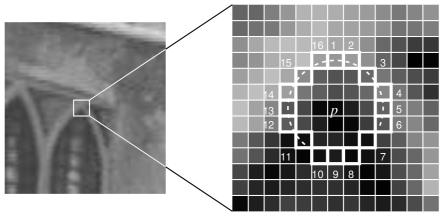
\includegraphics[width=0.7\linewidth]{figures/FASTcornerdetector}
	\caption{Detetor de canto FAST, circulo em volta do ponto \textit{p}. \cite{VisualOdometryRodasVehicles}}
	\label{fig:fastcornerdetector}
\end{figure}

Analisando a Figura  ~\ref{fig:fastcornerdetector} , os pixeis 11-16 e 1-6 têm maior intensidade que os pixel a examinar, pixel \textit{p}. Isto significa que o pixel \textit{p} é um canto. O teste realizado pode ser resumido a duas condições:
\begin{enumerate}
	\item Se existirem N pixeis adjacentes no anel na qual todos têm intensidade superior ao pixel \textit{p}, então \textit{p} é um canto.
	\item Se existirem N pixeis adjacentes no anel na qual todos têm intensidade inferior ao pixel \textit{p}, então \textit{p} é um canto.	
\end{enumerate}
Assim se alguma condição for verdadeira , o pixel \textit{p} é classificado como canto. O parâmetro N é usualmente 12 de forma a obter uma deteção com alta qualidade. N pode ser 9 de forma a detenção ser mais rápida. 
O algoritmo depende da intensidade de threshold , o qual em diferentes ambientes deve originar diferentes resultados e o threshold deve ser ajustado para a melhor performance. Desde que o algoritmo use um círculo de pixeis para determinar se o pixel examinado é um canto, o algoritmo é invariante à escala e rotação.


\subsection{Detectores de blobs}

\subsubsection{SIFT}

A diferença de gaussianas (DoG, do inglês \textit{Diference of Gaussians}) foi utilizada para identificar características invariantes à escala, rotação e parcialmente invariantes à variação na luminosidade e transformações afins. O método SIFT (do inglês, \textit{Scale Invariant Feature Transform}) é composto por um detetor de blobs baseado em DoG.

O primeiro passo no algoritmo de SIFT é utilizar a função gaussiana sobre uma imagem com escalas diferentes para gerar o espaço de escalas da imagem.

A função \begin{equation}\label{equaSIFTdet}
\textit{L}(x,y,\sigma) = \textit{G}(x,y,\sigma)*\textit{I}_{x,y} \end{equation}
define o espaço de escalas da imagem $\textit{I}_{x,y}$. Na equação ~\ref{equaSIFTdet}
, o operador * define a convolução da função gaussiana onde $\textit{I}_{x,y}$ é a imagem de entrada e o núcleo Gaussiano $\textit{G}(x,y,\sigma)$ é igual a  \[ G( \textit{x},\textit{y},\textit{$\sigma$}) =\ \frac{1}{2\pi\sigma^2} e^{-\frac{x^2 + y^2}{2\sigma^2}} . \]

O passo é repetido com diferentes $\sigma$, escalados por um fator $\textit{k}$. \[ \textit{D}(x,y,\sigma) = \textit{L}(x,y,\textit{k}\sigma) - \textit{L}(x,y,\sigma). \]

Desde que todas as DoG estão calculadas para a escala corrente , designada como oitava, a imagem cujo valor de $\sigma$ é duas vezes o valor de $\sigma$ inicial na oitava é selecionada para ser reproduzida. O processo é ilustrado na Figura ~\ref{fig:compitation-of-dog}.

\begin{figure}[h!]
	\centering
	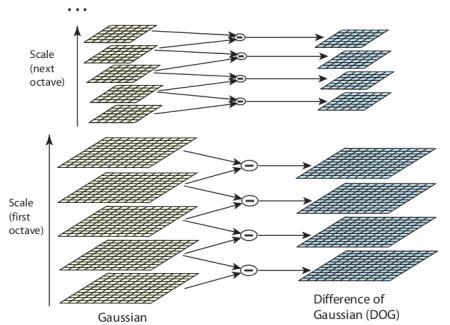
\includegraphics[width=0.7\linewidth]{figures/compitationofDoG}
	\caption{Computação da DoG. \cite{VisualOdometryRodasVehicles}}
	\label{fig:compitation-of-dog}
\end{figure}

Calculadas as DoGs, deseja-se obter os máximos e mínimos locais em todas as escalas de $\textit{D}(x,y,\sigma)$. Para isso avalia-se cada ponto da primeira oitava com seus 26 vizinhos, 8 no mesmo nível e 9 nos níveis superiores e inferiores de escala. A Figura ~\ref{fig:pixelcamadas} apresenta essa comparação. Se o ponto for extremo nessa oitava, sua posição é estimada na oitava seguinte e o processo é repetido para esse ponto. As informações referentes à escala e oitava alcançadas são guardadas e farão parte da característica. 


\begin{figure}[h!]
	\centering
	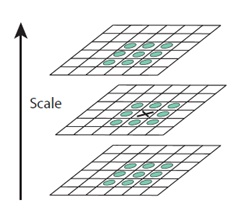
\includegraphics[width=0.5\linewidth]{figures/pixelCamadas}
	\caption{O \textit{pixel} marcado com um \textit{x} é avaliado em relação aos seus vizinhos no mesmo nível e nos níveis superiores e inferiores. \cite{VisualOdometryRodasVehicles}}
	\label{fig:pixelcamadas}
\end{figure}

Uma vez obtido o ponto de extremo é refinada a posição para obter uma posição em $\textit{subpixeis}$. è utilizada uma expansão de Taylor em torno do ponto de extremo \begin{equation}\label{equacao2.1}
D(x) = D + \frac{\partial D^T}{\partial x}x + \frac{1}{2}x^T\frac{\partial^2D}{\partial x^2}x
\end{equation} onde c é o deslocamento em torno do ponto de extremo. O ponto extremo $\hat{x}$ é determinado derivando a equação ~\ref{equacao2.1} em relação a x e igualando a zero. O resultado é dado por \begin{equation}\label{equacao2.2}
\hat{x} = -\frac{\partial^2D^{-1}}{\partial^2x^2}\frac{\partial D}{\partial x}. 
\end{equation} 
Se houver variação maior que 0.5 em qualquer uma das direções o ponto muda de pixel e o valor de extremo é interpolado no novo ponto. O valor do ponto de extremo é refinado para remover extremos com baixo contraste. Essa operação é feita substituindo a equação ~\ref{equacao2.2} na equação ~\ref{equacao2.1}, resultando em \[ D( \hat{x} ) = D + \frac{1}{2}\frac{\partial D^T}{\partial x} \hat{x} . \]

Outro filtro usa uma ideia semelhante para remover pontos de borda. A matriz hessiana \[ \textit{H} = \left[ \begin{array}{cc}
D_{xx} & D_{xy} \\ 
D_{xy} & D_{yy}
\end{array} \right]  \] descreve a curvatura principal da imagem em torno do ponto de extremo. Analisando a relação entre os autovalores de $\textit{H}$ avalia-se que se o determinante de \textit{H} é negativo o ponto é descartado. Assim a avaliação é feita sobre a relação dos autovalores, como mostra a seguinte equação: \begin{equation}\label{equacaoseg}
\frac{\textit{Tr}(H)^2}{\textit{Det}(H)} = \frac{(\alpha + \beta)^2}{\alpha\beta} = \frac{(r\beta + \beta)^2}{r\beta^2} = \frac{(r + 1)^2}{r}, 
\end{equation} 
onde $\alpha$ = $r\beta$. Um valor extremo será descartado caso a relação \[ \frac{\textit{Tr}(H)^2}{\textit{Det}(H)} < \frac{(\tau + 1)^2}{\tau}, \] para um limiar $\tau$ a ser definido.  

Até este ponto foram obtidas localizações e escalas dos pontos de extremos e foram removidos extremos com baixo contraste e em bordas. Resta obter uma orientação para o ponto. Para isso escolhe-se em cada oitava a imagem gaussiana \textit{L} cuja escala mais se aproxima da escala do ponto de extremo. Para cada uma das imagens $\textit{L}(x,y)$  (note que o valor de $\sigma$ não aparece pois é definido como o mesmo do ponto de extremo) a magnitude $\textit{m}(x,y)$ e a orientação $\theta$(x,y) são calculadas usando \[ \textit{m}(x,y) = \sqrt{(\textit{L}(x  +1,y) - \textit{L}(x - 1,y))^2 + (\textit{L}(x,y + 1) - \textit{L}(x,y - 1))^2} \] \[ \theta (x,y) = \textit{tan}^{-1}((\textit{L}(x,y +1) - \textit{L}(x,y - 1))/(\textit{L}(x + 1,y) - \textit{L}(x - 1,y))).\]
Calcula-se as orientações em torno do ponto de extremo e um histograma é montado com 36 orientações possíveis para a característica, cada um respondendo por 10º dos 360º possíveis para $\theta$(x,y). Cada uma das orientações $\theta$(x,y) é pesada utilizando a magnitude $\textit{m}(x,y)$ e uma janela gaussiana com $\sigma$ sendo 1.5 vezes a escala do ponto de extremo antes de ser adicionada à orientação da característica.

Picos no histograma das orientações em torno do ponto de extremo correspondem a direções dominantes do gradiente local. O maior pico de histograma é identificado e uma característica é gerada com localização, escala a e orientação. Picos no histograma que sejam máximos locais e cuja magnitude seja maior que 80\% da do pico máximo também geram características com a mesma localização e escala, mas com a orientação diferente. Por fim, para cada pico que gerou uma característica, uma parábola é traçada pelo pico e os dois valores do histograma adjacentes a ele. Para se obter maior precisão o pico máximo é então tomado como o máximo da parábola gerada pela interpolação dos três picos.


\subsubsection{SURF}

O detetor SURF (do inglês, \textit{Speeded Up Robust Features}) é similar ao SIFT no sentido que os passos são iguais, mas são feitos diferentemente. A imagem em analise é filtrada com janelas baseada no método do integral da imagem, como uma aproximação Gaussiana \begin{equation}\label{surfequation}
I_{\Sigma}(x,y) = \sum_{i}^{x}\sum_{j}^{y}{I(i,j)}. \end{equation}
O benefício do uso deste método é a redução do numero de cálculos e a diferença no tamanho da janela que influenciam no tempo de cálculos. Uma adição e duas subtrações usando os pontos de canto são requeridas para o calculo da soma, Figura ~\ref{fig:surfsqware}.

\begin{figure}[h!]
	\centering
	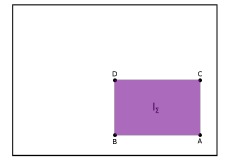
\includegraphics[width=0.4\linewidth]{figures/surfsqware}
	\caption{Ilustração do método do integral da imagem. \cite{VisualOdometryRodasVehicles}}
	\label{fig:surfsqware}
\end{figure}

A soma de todos os pixeis como visto em ~\ref{surfequation} é igual a \textit{$I_{\sum}$} = A - B - C + D, dado que a origem da imagem original é no canto superior esquerdo. Deteção blob é usado e é realizada usando a matriz Hessian. Através de uma imagem \textit{I} e um ponto \textbf{x} = (x,y) na imagem, a matriz Hessian $\textit{H}(x,\sigma)$ é calculada. Onde $\sigma$ é a escala atual. \[  \textit{H}(x,\sigma) = \left[ \begin{array}{cc}
L_{xx}(x,\sigma) & L_{xy}(x,\sigma) \\ 
L_{xy}(x,\sigma) & L_{yy}(x,\sigma)
\end{array} \right]. \] 
Onde $\textit{L}_{xx,xy,yy}(x,\sigma)$  são as derivadas de segunda ordem no ponto x da imagem \textit{I}. Estas derivadas parciais são aproximadas usando filtros para diferentes escalas e oitavas. Depois de suavizar e reduzir a amostragem da imagem para cada $\sigma$ como no algoritmo SIFT, o algoritmo SURF aumenta o tamanho do filtro. Uma vez que o Hessian é formado para o ponto \textbf{x} numa certa escala $\sigma$, o determinante do Hessian é calculado e ponderado de forma a obter a melhor aproximação.  O determinante aproximado é guardado em um mapa de resposta para a escala atual.
Uma vez calculada a matriz Hessian para todas as oitavas, o algoritmo procura o máximo local e o máximo detetado é guardado e interpolado na escala e no espaço da imagem. 

Assim, o detetor de SURF têm pontos chaves:
\begin{itemize}
	\item Localização
	\item Escala
	\item Orientação
\end{itemize}


\section{Descritor de Características}

Como mencionado anteriormente, uma boa característica tem como propriedade a diferenciabilidade. A diferenciabilidade permite que a característica seja identificada de maneira única. Porém se for utilizado somente o ponto de interesse onde localiza-se a característica, a diferenciação torna-se difícil, uma vez que existe pouca informação para gerar um identificador para aquele ponto.

Desta forma, os descritores codificam uma área da imagem em torno do ponto característico, para cada ponto característico. Ao fazer isto, os pontos característicos entre duas imagens são comparáveis uns com os outros.


\subsection{ORB}

O descritor ORB (do inglês, \textit{Oriented FAST and Rotation-Aware BRIEF}) precisa de pontos característicos para serem detetados pelo detetor oFAST. A deteção é realizada como descrita na secção ~\ref{fastsection} com a adição da orientação do ponto característico. Isto é realizado calculando o centroide de intensidade. Primeiro, o momento do patch é calculado como \[ \textit{$m_{pq}$} = \sigma \textit{$ x^py^qI$}(x,y) ,\]
onde \textit{p} e \textit{q} são parâmetros dos pixeis em ordem do momento. E o centroide do patch é encontrado com a seguinte equação \[ C = ( \frac{ \textit{m}_{10} }{ \textit{m}_{00}} ,  \frac{ \textit{m}_{01} }{ \textit{m}_{00}} ) . \]
Em seguida o vetor $\vec{OC}$ é construido do ponto central do ponto de característica, O, para o centroide obtido anteriormente, C. O ângulo de $\vec{OC}$ é obtido com a orientação do patch. \[ \theta = atan^2( \textit{m}_{01},\textit{m}_{10}) . \]
Uma vez atribuída uma orientação ao ponto característico, o descritor BRIEF (do inglês, \textit{Binary Robust Independent Elementary Features}) realiza um teste binário, $\tau$, da intensidade entre pontos de um patch de imagem suavizada. O teste é definido como  \[\sigma\left(p;x,y\right) = \left\{\begin{array}{cc}
1, & p(x)<p(y) \\ 
0, & p(x) \geq  p(y)   
\end{array}\right.
,\]
onde \textbf{p} é o patch de imagem que foi suavizada e \textbf{$(x,y)$} é o ponto de teste.
O resultado da característica é um vetor de 256 testes binários \[ f_{256} \left( p \right) = \sum_{1\ \le\ i\ \le\ 256\ } {2^{i-1}\tau\left(p;x_i,y_i\right) } . \]

De forma a realizar um descritor de recurso elementares independentes robustos binários (BRIEF) invariantes à rotação, é orientar o descritor para a orientação $\theta$ dos pontos caraterísticos. Isto é feito construindo uma versão direcionada dos testes binários na localização do recurso \[ \textbf{$\textbf{S}_{\theta} = \textbf{R}_{\theta}\textbf{S}$} ,\] onde \textbf{$\textbf{R}_{\theta}$} é a matriz rotação e \textbf{S} é igual a : \[ \textbf{S} = \left[ \begin{array}{ccc}
\textbf{x}_1 & ... & \textbf{x}_{256}\\
\textbf{y}_1 & ... & \textbf{y}_{256}
\end{array} \right] . \]

Desta forma , o BRIEF dirigido é igual a : \[ g_n(\textbf{p},\theta) = f_n(\textbf{p})|(\textbf{x}_i,\textbf{y}_i) \in S_{\theta} .\]


Uma desvantagem com o BRIEF dirigido é a baixa variação e alta correlação entre os testes binários. Isso é reduzido pela busca entre os testes binários para testes com alta variação e não correlação. 	

\subsection{SIFT}

Primeiro o gradiente e a orientação são analisados para os pontos numa janela que é centrada pelo ponto característico. O tamanho da janela é 16 x 16 caixas em uma matriz. Esta matriz é dividida em 4 x 4 sub-regiões, onde o histograma baseado na orientação é construído para cada região. Em seguida, as coordenadas desses pontos e orientações do gradiente são rodadas de forma a incorporar a invariância rotacional. Os pontos são futuramente aperfeiçoados por uma função Gaussiana com peso $\sigma$ = $\frac{w}{2}$, onde \textit{w} é o tamanho da janela do descritor. Como ilustra a Figura ~\ref{fig:siftdescriptor}

\begin{figure}[h!]
	\centering
	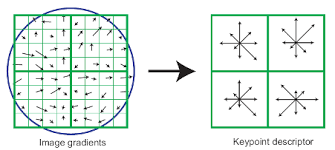
\includegraphics[width=0.7\linewidth]{figures/SIFTdescriptor}
	\caption{Descritor SIFT. As setas designam a soma dos gradientes nas caixas individuais. O círculo azul representa a região que é considerada na atuação do filtro Gausiano. Este exemplo ilustra uma matriz 8x8 resultando num 2x2 descritor. \cite{VisualOdometryRodasVehicles}}
	\label{fig:siftdescriptor}
\end{figure}

\subsection{SURF}

Uma janela quadrada é centrada no ponto de característica, com a mesma orientação. O tamanho da janela é 20\textit{s} x 20\textit{s} , onde \textit{s} é a escala onde o ponto característico foi detetado. De seguida, a janela é dividida em sub-regiões 4 x 4 . As respostas das ondas de Haar e seu valor absoluto são resumidas para direção horizontal e vertical em cada sub região. O descritor resultante consiste em um vetor 4D que contém as quatro somas para cada sub-região.


\section{Associação de Características}

O processo de correspondência de características é um requisito para muitas aplicações relacionadas com imagens, tais como, recuperação de uma imagem, deteção do movimento e reconstrução da forma. 
Como mencionado no início da Secção ~\ref{detCar}, espera-se que uma boa característica tenha como propriedade a diferenciabilidade. A diferenciabilidade permite que a característica seja identificada (idealmente) de maneira única.
As diferentes características determinadas pela etapa anterior precisam ser correspondidas, ou seja, é preciso determinar quais características são as mesmas em imagens distintas. Geralmente existem dois métodos diferentes para encontrar suas correspondências: correspondência de características e seguimento de características. 


\subsection{Correspondência de Características}

O método de correspondência de características consiste na deteção de características de maneira independente em todas as imagens com um determinado detetor de características.
Idealmente, as correspondências detetadas representam a mesma informação nas imagens.
Depois são efetuadas as correspondências entre as características detetadas usando uma estratégia de comparação baseada em medidas de semelhança.
Este método é muito usado em ambientes exteriores de grandes dimensões, em que as imagens são capturadas partir de posições distantes entre si, com a finalidade de limitar os problemas relacionados com desvio de movimento.

\subsubsection{Brute force}\label{subchap:BRUTE}

O método \textit{Brute force} compara um descritor de um conjunto de pontos caracteristicos da primeira image com todos os descritores dos pontos caracteristicos da segunda imagem. Geralmente, o descritor com pequena distância Euclidiana é comparado com o descritor da primeira imagem. A distância do descritor é limitada por um threshold de forma a tornar a comparação válida. O tempo entre duas imagens devem ser pequenas de forma à comparação do descritor ser correta.


\subsection{Seguimento de Características}

O método de seguimento de características, com alternativa, deteta características em apenas uma imagem com um determinado detetor de características. Na próxima imagem a característica correspondente é procurada na área em torno da localização da característica detetada.
Este método de deteção e seguimento é muito usado em ambientes interiores de pequenas dimensões e é adequado para aplicações de OV. 
Uma vez que as imagens são capturadas a partir de posições próximas e a quantidade de movimentos entre imagens sucessivas geralmente é pequena. 

\subsubsection{FLANN}\label{subchap:FLANN}

O método FLANN (do inglês, \textit{Fast Library for Approximate Nearest Neighbours}) é considerado um algoritmo que procura correspondência dos descritores numa vizinhança próxima do ponto característico.  O OpenCV utiliza uma correspondência baseada no FLANN que utiliza a estrutura de dados da árvore k-d e vizinhos próximos. K-d significa \textit{k} dimensões, onde \textit{k} é um inteiro positivo. A ideia base é :
\begin{itemize}
	\item Escolher uma dimensão \textit{k}.
	\item Encontrar o valor mediano dessa dimensão.
	\item Dividir a dimensão em duas partes com base no valor mediano.
	\item Repetir, até k-1 atingir 0 e começar de novo com k original até que todos elementos no conjunto de dados sejam examinados.
\end{itemize}

O processo é ilustrado na figura ~\ref{fig:flann} . Este exemplo inicia-se no ponto (7,2).

\begin{figure}[h!] %colocar figura a seguir ao texto anterior
	\begin{center}
		\leavevmode		
		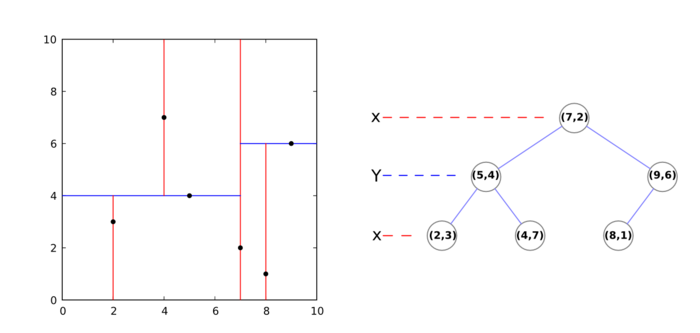
\includegraphics[width=0.8\textwidth]{flann}
		\caption{A imagem da esquerda ilustra a decomposição 2-d, note que as linhas vermelhas são para o eixo x e as linhas azuis para o eixo y. A imagem da direita ilustra a árvore 2-d correspondente.}
		\label{fig:flann}
	\end{center}
\end{figure}

Uma vez que a árvore k-d é formada, o próximo passo é usar pontos do segundo conjunto de dados e ver em qual nó da árvore k-d que o ponto examinado está mais próximo. O procedimento é chamado vizinho mais próximo (NN, do inglês, \textit{Nearest Neighbour}). Começando no nó raiz (7,2), como ilustrado, o algoritmo percorre a árvore 2-d construída recursivamente. Escolhe o nó da esquerda ou direita se o ponto examinado tiver um valor maior ou menos que o nó atual na dimensão atual, respetivamente. Uma vez que o algoritmo tenha atingido um nó final, o algoritmo guarda esse nó como o melhor atualmente. A recursão é então finalizada e o algoritmo começa a atravessar de volta ao nó raiz. A distância até ao ponto examinado é verificada em cada nó, se a distância for menor então é atualizado o melhor valor. O algoritmo também verifica se o hiperplano do outro lado da árvore está dentro do raio da menor distância atual, se não , esse hiperplano é descartado. Se estiver dentro, o algoritmo percorre esse ramo da árvore k-d também. O procedimento pode ser visto na figura ilustrada ~\ref{fig:flannNN}.

\begin{figure}[h!] %colocar figura a seguir ao texto anterior
	\begin{center}
		\leavevmode		
		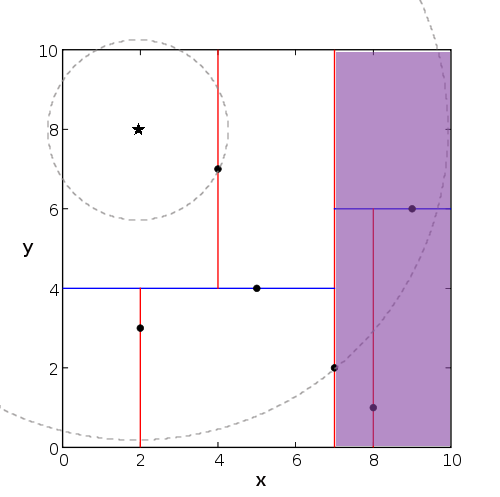
\includegraphics[width=0.6\textwidth]{flannNN}
		\caption{Algoritmo de procura NN baseado nas árvores 2-d.}
		\label{fig:flannNN}
	\end{center}
\end{figure}

O ponto (2,8) é examinado para o seu vizinho mais próximo, marcado com uma estrela na figura. O algoritmo começa no nó raiz (7,2) e a distância , isto é , o raio do grande circulo centrado na estrela cobre todos os hiperplanos. Isso significa que não podemos descartar nenhum hiperplano. O algoritmo percorre a árvore, ignorando os hiperplanos roxos da figura. O nó da folha (4,7) é definido como o melhor e o algoritmo começa a atravessar de volta para o nó raiz, verificando a distância em cada nó. Desde que o raio do pequeno círculo centrado em torno da estrela é a melhor combinação atual e não está se cruzando com os hiperplanos roxos, pode-se descartar esses hiperplanos e o algoritmo não procura por eles. Uma vez no nó raiz, o algoritmo termina e (4,7) era de fato o mais próximo vizinho.

\section{Estimação do movimento}

A etapa de estimação do movimento representa o núcleo da computação em um sistema de OV. Ela efetua o cálculo do movimento da câmara entre a imagem atual e a imagem anterior. A trajetória da câmara e do agente (assumindo que estão ligados rigidamente) pode ser recuperada completamente através da concatenação de todos os movimentos individuais.

Esta secção explica com a transformação relativa \textit{$T_k$} pode ser calculada entre duas imagens \textit{$I_{k-1}$} e \textit{$I_k$} a partir de dois conjuntos de pontos característicos correspondentes \textit{$f_{k-1}$} , \textit{$f_k$} nos instantes de tempo \textit{k - 1} e \textit{k}, respetivamente. Existem três métodos diferentes para o cálculo do \textit{$T_k$} dependendo se as correspondências dos pontos característicos são especificadas em três ou duas dimensões. Os métodos referidos são:


\begin{itemize}
	\item 2D-para-2D: Neste caso, ambos \textit{$f_{k-1}$} e \textit{$f_k$} são especificados pelas coordenadas 2D da imagem.
	\item 3D-para-3D: Neste caso, ambos \textit{$f_{k-1}$} e \textit{$f_k$} são especificados pelas coordenadas 3D da imagem. Para realizar esta acção, é necessário a triangulação de pontos 3D em cada instante de tempo, isto pode ser feito a partir de um sistema com câmaras estéreo, por exemplo.
	\item 3D-para-2D: Neste caso, \textit{$f_{k-1}$} são especificados em 3D e \textit{$f_k$} são as suas correspondentes reprojeções em 2D na imagem \textit{$I_k$}.No caso da utilização de um sistema monocular, a estrutura 3D necessita de triangular duas câmaras adjacentes (isto é \textit{$I_{k-2}$} e \textit{$I_{k-1}$}) e assim a construção da imagem 2D . 
\end{itemize}



\subsection{2D-para-2D}

A relação geométrica entre duas imagens \textit{$I_k$} e \textit{$I_{k-1}$} da calibração da câmara é descrita pela matriz essencial \textit{E}. Esta contém os parâmetros de movimento da câmara para um fator de escala desconhecido. \[ E_k\ \approx\ {\hat{t}}_kR_k \] onde \textit{$t_k$} = $[ \textit{$t_x$}, \textit{$t_y$}, \textit{$t_z$} ]^T$ e \[ \hat{t}_k =\ \left[\begin{array}{ccc}0&-t_z&t_y\\t_z&0&-t_x\\-t_y&t_x&0\\\end{array}\right] . \]

A correspondência dos pontos característico, rotações e translações podem ser obtidos através da matriz essencial. A principal propriedade da estimação de movimento através de 2D-para-2D é a restrição epipolar, que determina a linha em cada ponto de característica correspondente em outra imagem, como ilustrado na Figura ~\ref{fig:epipolarconstrait}.

\begin{figure}[h!]
	\centering
	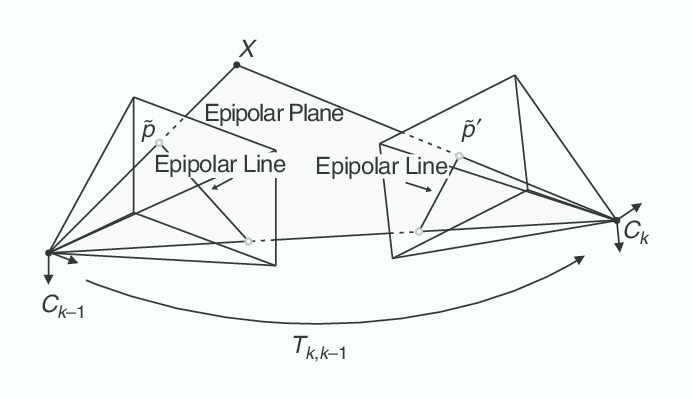
\includegraphics[width=0.7\linewidth]{figures/equipolarline}
	\caption{Uma ilustração da restrição epipolar. \cite{VOpart1}}
	\label{fig:epipolarconstrait}
\end{figure}

Esta restrição pode ser formulada por $p'^{T}$Ep = 0, onde p é um ponto característico numa imagem e $p'$ é o correspondente ponto característico noutra imagem.

Através da estimação da matriz \textit{E}, a rotação e translação pode ser extraída. 
\[ R = U(\pm W^T)V^T ,\] \[ \hat{t} =  U(\pm W)SU^T, \] 
onde \[  W^T = \left[\begin{array}{ccc}0&\pm1&0\\\mp1&0&0\\0&0&1\\\end{array}\right] \] 
e U, S, V são obtidas através do USV (do inglês, \textit{Singular Value Decomposityon}) \[ E = USV^T \]

Para recuperar a trajetória de uma sequência de imagens é necessário a concatenação das diferentes transformações \textit{$T_{0:n}$}. Para isso é necessário uma escala relativa obtida através de : \[ r = \frac{ \| X_{k-1,i} - X_{k-1,j} \| }{ \| X_{k,i} - X_{k,j} \| } \] 

Desta forma, o algoritmo de OV com correspondência 2D-para-2D é sumariado de seguida:
\begin{enumerate}
	\item Capturar uma imagem \textit{$I_{k}$}.
	\item Extrair e conjugar pontos característicos entre \textit{$I_{k-1}$} e \textit{$I_{k}$}.
	\item Obter a matriz essencial do par de imagens \textit{$I_{k-1},I_k$}.
	\item Decompor a matriz essencial em \textit{$R_k$} e \textit{$\hat{t}_k$}.
	\item Computorizar a escala relativa \textit{$\hat{t}_k$}.
	\item Concatenar a transformação $C_k$ = $C_{k-1}$ $T_k$.
	\item Repetir 1.
\end{enumerate}


\subsection{3D-para-3D}

A estimação do movimento através da correspondência 3D-para-3D é usada em sistemas estéreo. 

A solução geral é encontrar \textit{$T_k$} que minimiza a distância \textit{$L_2$} entre duas 3D características \[ \arg_{\ T_k}^{min}\sum_{i}{\left \| \tilde{X}_k^i - T_k\tilde{X}_{k-1}^i \right \|} \] 
onde \textit{i} é a característica \textit{i} e \textit{$X_{k},X_{k-1}$} são as coordenadas homogéneas dos pontos 3D. 

Como analisado anteriormente, o número mínimo de soluções são três correspondências não colineares. Desta forma, se n $\geq$ 3, uma solução possível é realizar a diferença dos centroides das características 3D e uma rotação usando SVD. A translação é dada por \[ t_{k\ }=\ {\bar{X}}_k\ -\ R{\bar{X}}_{k-1} \] onde - é a média aritmética.

A rotação é eficientemente calculada através do SVD como \[ R_k = VU^T \] onde $USV^T$ = $svd({(X_{k-1}\ -\ {\bar{X}}_{k-1})(X_k\ -\ {\bar{X}}_k)}^T)$ e \textit{$X_k$} corresponde ao ponto 3D.

O algoritmo de OV com correspondência 3D-para-3D é sumariado de seguida:
\begin{enumerate}
	\item Capturar duas pares de imagens num sistema estéreo, \textit{$I_{l,k-1}$},\textit{$I_{r,k-1}$} e \textit{$I_{l,k}$},\textit{$I_{r,k}$}
	\item Extrair e conjugar pontos característicos entre \textit{$I_{l,k-1}$} e \textit{$I_{l,k}$}
	\item Triangular os pontos característicos conjugados para cada par de estéreo.
	\item Computacional \textit{$T_k$} de pontos característicos 3D, \textit{$X_{k-1}$} e \textit{$X_k$}  
	\item Concatenar a transformação $C_k$ = $ C_{k-1}$ $T_k$
	\item Repetir 1
\end{enumerate}



\subsection{3D-para-2D}

A estimação do movimento de 3D-para-2D é mais precisa do que 3D-para-3D porque são minimizados os erros de reprojeção. A transformação \textit{$T_k$} é analisada num sistema estéreo através do \textit{$X_{k-1}$} e \textit{$p_k$}. No caso de um sistema monocular, através da triangulação das medições de imagens \textit{$p_{k-1}$} e \textit{$p_{k-2}$}. 

A formula general neste caso é encontrar \textit{$T_k$} que minimize o erro de reprojeção da imagem \[ \arg_{\ T_k}^{min} \sum_{i}{\left \| p_k^i - \hat{p}_{k-1}^i \right \|}^2 \]
onde \textit{$p_{k-1}$} é a reprojeção do ponto 3D \textit{$X_{k-1}^i$} na imagem \textit{$I_k$} de acordo com a transformação \textit{$T_k$}. 

Como no problema da correspondência 3D-para-3D são necessários um número mínimo de pontos. Com um número de pontos igual a 6, P é calculado através do uso de SVD e a rotação e translação é obtida através de $P_k$ = [R|t]. 

Assim, a estimação através de 3D-para-2D assume que os pontos são obtidos de apenas uma câmara. Desta forma, num sistema estéreo o ponto 2D é obtido através da junção da câmara da esquerda com a câmara da direita. Obviamente a captura das imagens têm de ser no mesmo instante de tempo.  Para o caso de um sistema monocular é algoritmo inicializa após a captura das duas primeiras imagens, desta forma é necessário triangular duas imagens capturadas em instantes diferentes para obter o ponto.

O algoritmo de OV com correspondência 3D-para-2D é sumariado de seguida:
\begin{enumerate}
	\item Realizar na primeira vez:
	\begin{enumerate}[label*=\arabic*.]
		\item Capturar duas imagens \textit{$I_{k-2}$},\textit{$I_{k-1}$} 
		\item Extrair e conjugar pontos característicos entre eles
		\item Triangular os pontos característicos \textit{$I_{k-2},I_{k-1}$}
	\end{enumerate}
	\item Realizar a cada iteração:
	\begin{enumerate}[label*=\arabic*.]
		\item Capturar nova imagem \textit{$I_k$}
		\item Extrair e conjugar pontos característicos com a imagem anterior \textit{$I_{k-1}$}
		\item Computorizar posição da câmara através do calculo 3D-para-2D
		\item Triangular todos os novos pontos característicos entre \textit{$I_k$} e \textit{$I_{k-1}$}
		\item Repetir 2.1
	\end{enumerate}
	
\end{enumerate}




\section{Métodos de ajuste de erros}

A associação de pontos , usualmente, está contaminada por \textit{outliers}\footnote{valor atípico, é uma observação que apresenta um grande afastamento das demais series ou é inconsistente.}, isto é, associação de dados errada. As possíveis causas de \textit{outliers} são ruídos da imagem, exclusões, pouca nitidez, alteração de posições e iluminação das quais os modelos matemáticos dos detetores de características não detetam. 

Para  a estimação da movimentação correta da câmara é importante que o \textit{outliers} sejam removidos. 

\subsection{Windowed bundle adjustment}

O \textit{bundle adjustment} é um algoritmo criado no campo da fotometria em meados da década de 1950 e tornou-se muito utilizado no campo da visão por computador, explicitamente na área de reconstrução 3D.

A função principal é tentar otimizar ao mesmo tempo os parâmetros (intrínsecos e extrínsecos) da câmara, bem como os parâmetros dos pontos 3D de referência. Ele é aplicado para os casos em que as características detetadas numa imagem são procuradas em mais do que duas características. Este algoritmo considera uma "janela" de \textit{n} características da imagem e depois faz uma otimização dos parâmetros das posições da câmara e dos pontos 3D de referência para este conjunto de características da imagem.

No \textit{bundle adjustment}, a função de erro a minimizar é o erro de reprojeção da imagem. 
\[ \arg_{X^i,C_k}^{min} \sum_{i,k}{\left \| p_k^i - g(X^i ,C_k) \right \|}^2 ,\]
onde $p_k^i$ é o i-ésimo ponto da imagem dos pontos 3D de referência \textit{$X^1$} medido na k-ésima imagem e $\textit{g}(X^i,C_k)$ é a sua imagem de reprojeção de acordo com a posição atual da câmara $C_k$. O erro de reprojeção é uma função não-linear.

Para concluir, o principal objetivo do \textit{bundle adjustment} em sistemas de OV é a redução do desvio entre a trajetória estimada e a real.

\subsection{RANSAC}


Tal como referido anteriormente, uma das funções do algoritmo RANSAC é a remoção dos \textit{outliers}, que permite a estimação do movimento da câmara de uma forma mais precisa. A etapa de rejeição dos \textit{outliers} é a mais delicada em sistema de OV.

De uma forma geral, este algoritmo é utilizado quando se pretende estimar um modelo (por exemplo os parâmetros de rotação e translação de uma câmara) na presença de \textit{outliers}.

A ideia fundamental do RANSAC é calcular candidatos modelo a partir de amostras de conjuntos de pontos de dados. A escolha das amostras é feita aleatoriamente. Posteriormente com os outros dados é selecionada como solução.

O esboço deste algoritmo é apresentado em seguida:

%%Inserir figura de algoritmo

O número de iterações N necessário para garantir a solução correta é calculado pela equação

\[  N = \frac{log(1-p)}{log(1-(1-\epsilon)^s)} \]

O valor \textit{s} representa o número de pontos de dados a partir do qual o modelo pode ser instanciado, $\epsilon$ é a percentagem de \textit{outliers} nos pontos de dados e \textit{p} representa a probabilidade de sucesso pretendida.

Notar que o algoritmo é um método iterativo e não determinístico de tal forma que calcula uma diferente solução em cada execução. Contudo, a solução tende a estabilizar à medida que o número de iterações aumenta.

%	\chapter{Caracterização do problema}\label{chap:chap4}

Para obter o conhecimento da localização através de OV é necessário calcular a distância entre duas imagens consecutivas. De forma a obter a distância, necessitamos de pontos caraterísticos nas imagens para ser possível a sua deteção na imagem seguinte. Tal, é possível através do conhecimento da formação de uma imagem.

Devido ao meio ambiente em que este projeto está incorporado , a obtenção de imagens com ângulos de cerca 45º (ângulo comum de uma câmara)  limita muito a deteção de pontos caraterísticos. De forma a diminuir esta desvantagem utiliza-se uma lente olho de peixe, com abertura de cerca de 180º para obtenção de  uma maior qualidade e quantidade de pontos caraterísticos. 

Como analisado no capitulo ~\ref{chap:odometria visual}, já existem vários métodos de deteção, associação de pontos caraterísticos e estimação do movimento. Maior parte destes métodos são implementados em câmaras do tipo pinhole , sem distorções. No artigo \cite{6460718}, os autores comparam os vários tipos de detetores e descritores para vários métodos, obtendo tempos de execução para cada método. Em outro artigo, \cite{ImagMatch}, os autores adicionam rotações e distorções às imagens de forma a comparar a eficácia dos métodos. Mas, como analisado em \cite{Zhang2016}, o uso de lentes olho de peixe adiciona muitos benefícios.  Nos artigos, \cite{Forster2014,Forster2017} , os autores implementaram OV em UAVs. Desta forma, torna-se importante a realização do estudo para que ocorra a implementação em  robôs agrícolas com câmaras com lente olho de peixe e sistema monocular.

%	\chapter{Plano de Trabalho} \label{chap:concl}

Neste capítulo, serão apresentadas as principais tarefas de desenvolvimento do projeto, a metodologia adotada e as ferramentas utilizadas. Na Figura ~\ref{fig:gantt} podemos ver um diagrama de \textit{Gantt} referente às principais tarefas a realizar:

\begin{figure}[h!]
	\begin{ganttchart}[y unit title=0.4cm,
	y unit chart=0.5cm,
	vgrid,hgrid,
	title height=1,
	bar/.style={draw,fill=cyan},
	bar incomplete/.append style={fill=yellow!50},
	bar height=0.7]{1}{24}
	\gantttitle{Fevereiro}{4}
	\gantttitle{Março}{4}
	\gantttitle{Abril}{4}
	\gantttitle{Maio}{4}
	\gantttitle{Junho}{4}
	\gantttitle{Julho}{4} \\
	\ganttbar{Fase 1}{1}{3} \\
	\ganttbar{Fase 2}{4}{6} \\
	\ganttbar{Fase 3}{7}{12} \\
	\ganttbar{Fase 4}{13}{18} \\
	\ganttbar{Fase 5}{19}{21} \\
	\ganttbar{Conclus\~ao}{22}{24} \\
	% rela\c c\~oes
	\ganttlink{elem0}{elem1}
	\ganttlink{elem1}{elem2}
	\ganttlink{elem2}{elem3}
	\ganttlink{elem3}{elem4}
	\ganttlink{elem4}{elem5}
	
\end{ganttchart}

	\caption{Diagrama de \textit{Gantt} com o planeamento do tempo para as principais tarefas.}
	\label{fig:gantt}
\end{figure}


\begin{enumerate}
	\item Fase 1: Obter uma comunicação entre a câmara e o raspberry pi através do uso de ROS (do inglês, \textit{Robot Operating System}), de forma a não limitar o uso da câmara nem do raspberry pi.
	\item Fase 2: Implementar os métodos analisados nos capítulos anteriores.
	\item Fase 3: Calcular a distância entre as imagens através do conhecimento da formação de uma imagem e realizar testes.
	\item Fase 4: Implementar os métodos em diferente câmaras , tais como FLIR (do inglês, \textit{Forward Looking Infra-Red} ) devido, ao facto, de o projeto RoMoVi já ter incorporado uma para deteção de troncos.
	\item Fase 5: Testes finais.
	\item Fase 6: Escrita da tese.
\end{enumerate}

A metodologia adotada consiste em implementar os métodos já existentes e realizar ajustes para o caso das câmaras com lentes de olho de peixe. 

Em termos de ferramentas a utilizar, será necessário a utilização de ROS (do inglês, \textit{Robot Operating System}), este fornece bibliotecas e ferramentas para ajudar os desenvolvedores de software a criar aplicações para robôs. A implementação deste software será em C/C++ desenvolvidas usando um \textit{IDE} sendo o eclipse o escolhido. Além disto, é necessário o uso de \textit{OpenCV}, uma biblioteca multiplataforma de forma a desenvolver os algoritmos de deteção , associação de pontos característicos e estimação do movimento.

Por último, a escrita é realizada na ferramenta \textit{Latex} , ideal para desenvolver documentos científicos devido à sua alta qualidade tipográfica.
	% !TeX spellcheck = pt_PT
\chapter{Sistema de Odometria Visual} \label{chap:sist}

Neste capitulo serão apresentados os procedimentos implementados para a realização dos testes. O capítulo aborda o \textit{software} e \textit{hardware} utilizados no desenvolvimento.

\section{Software}

Neste subcapítulo serão descritas as ferramentas de \textit{software} utilizadas assim como o código produzido.

\subsection{ROS}

ROS (\textit{Robot Operating System}) é uma \textit{framework} para desenvolvimento de \textit{sofware} de robótica. ROS consiste num compêndio de bibliotecas, ferramentas e outros recursos que visa facilitar a criação de comportamentos complexos alcançando uma vasta gama de plataformas robóticas distintas. 

O ROS fornece serviços idêntico a um sistema operativo, incluindo abstração de \textit{hardware}, baixo nivel de controlo, implementação de funcionalidades e mensagens que são transmitidas entre nós. Além disto , é constituido por bibliotecas e ferramentas para obter, criar, gravar e executar código em vários computadores. 

Desta forma, ROS  é caracterizado por :

\begin{itemize}
	\item \textbf{Pacotes} - O \textit{software} desenvolvido em ROS organiza-se em pacotes. Os pacotes são módulos que podem conter nós, bibliotecas independentes, \textit{datasets}, ficherisos de configuração, elementos de \textit{softwares} de terceiros, entre outros elementos que constituem o módulo. Os pacotes constituem a unidade base de compilação.
	\item \textbf{Nós} - Os nós são processos em ROS que executam computação, funcionando como programas. Os nós comunicam entre si através da publicação e subscrição de mensagens, serviços e através do \textit{Parameter Server}. Um sistema robótica em execução utiliza um conjunto de nós que cooperam para o seu funcionamento. A arquitectura distribuída de ROS permite que os nós em execução não necessitem de operar no mesmo equipamento, possibilitando a simbiose de diferentes plataformas comunicando entre si. O nó mestre pertence ao conjunto de nós laçando pelo \textit{roscore}, e tem a função de possibilitar aos nós que se localizem uns aos outros permitindo o estabelecimento de comunicações. 
	\item \textbf{Tópicos} - Os tópicos são os recipientes através dos quais os nós trocam mensagens  entre si. Os tópicos utilizam um modelo de publicação/subscrição que separa a produção de informação do seu consumo. Os nós não têm conhecimento de outros nós que publiquem determinado tópico ou o subscrevam. Um nó apenas necessita de subscrever os dados específicos a um tópico ou de publicar dados num tópico específico. A estrutura permite a existência de múltiplos publicadores e subscritores associados a cada tópico.
	\item \textbf{Serviços} - A unidirecionalidade existente no modelo publicador/subscritor não possibilita interações do tipo "pedido/resposta". Para possibilitar este tipo de interações existem os serviços em ROS. Um serviço é composto por um par de mensagens, uma mensagem definida para o pedido e outra para a resposta. Um nó pode oferecer um serviço ativado por um nó cliente ao submeter a mensagem de pedido.
 
\end{itemize}

A biblioteca de ROS suporta o desenvolvimento ROS em linguagem C++ e Python.

\subsubsection{Desenvolvimento em ROS}

- visodoAgro

	O algoritmo implementado neste nó pode ser resumido ao "seguinte"(mudar para figure) diagrama de atividade.
	
	
	Desta forma, no primeiro frame o algoritmo lê a imagem e transforma em escala de cinzas e de seguida calcula os pontos característicos desta. Sendo o primeiro frame não é possível realizar uma correspondência com o frame anterior, devido à inexistência deste.
	Desta forma, o algortimo avança para o próximo frame. A partir do segundo frame os passos são sempre iguais. Assim, o algoritmo obtêm a próximo frame e extraí a image em escala de cinzas, de seguida, caso se utilize o método de brute force , explicito no capitulo ~\ref{subchap:BRUTE}, é necessário calcula os pontos característicos deste frame e de seguida realizar a correspondência entre pontos característicos do frame atual e do anterior. Caso o método seja FLANN, explicito no capitulo ~\ref{subchap:FLANN}, é procurado o ponto característico no frame atual, numa pequena região à volta do pontos característico do frame anterior, que corresponde.
	
	Obtido a matriz com as devidas correspondências é necessário calcular a matriz Fundamental. Esta, é obtida através de um loop em que escolhe um conjunto de correspondências aleatoriamente de forma a calcular a matriz fundamental. De seguida testa a qualidade dessa matriz Fundamental através do numero de inliers, guardando o conjunto de correspondências com maior número de inliers. No fim calcula a matriz Fundamental com o melhor conjunto de correspondência.
	
	%\textbf{Expressar como a matriz fundamental é calculada.}
	
	\begin{figure}[h!] %colocar figura a seguir ao texto anterior
		\begin{center}
			\leavevmode		
			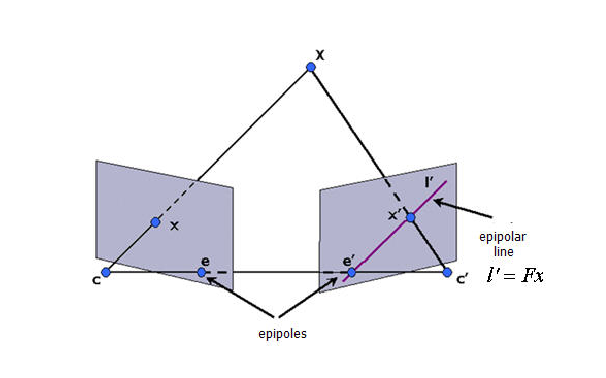
\includegraphics[width=0.6\textwidth]{epipolar.png}
			\caption{Representação da linha epipolar.}
			\label{fig:equ}
		\end{center}
	\end{figure}

	Como representado na figura ~\ref{fig:equ} o ponto \textbf{x} corresponde ao ponto no plano de imagem do frame anterior, \textbf{x'} corresponde ao ponto no plano de imagem do frame atual que corresponde os dois ao ponto \textbf{X} no mundo. Desta forma, \textbf{Fx} descreve uma linha (linha epipolar) na qual o ponto correspondente \textbf{x'} na outra imagem deve estar. Isto significa que, para todos os pares de pontos correspondentes : \[ {x}'^{T} F x = 0 \] 
	sendo, \[ F =  \left[ \begin{array}{ccc}
	f_{11} & f_{12} & f_{13} \\ 
	f_{21} & f_{22} & f_{23} \\ 
	f_{31} & f_{32} & f_{33} 
	\end{array}\right], \] \[ {x}' = \left[ \begin{array}{ccc}
	{u}' \\ {v}'\\ 1 
	\end{array} \right] e  \] \[ x = \left[ \begin{array}{ccc}
		u \\ v \\ 1  \end{array}\right]  . \]
		
	Desenvolvendo, obtemos : \[ u'uf_{11} + u'vf_{12} + u'f_{13} + v'uf_{21} + v'vf_{22} + v'f_{23} + uf_{31} + vf_{32} + f_{33} = 0 \]
	
	\[	\Leftrightarrow (u'u , u'v , u' , v'u , v'v , v' , u , v , 1) \left( \begin{array}{ccccccccc}
		f_{11}\\
		f_{12}\\
		f_{13}\\
		f_{21}\\
		f_{22}\\
		f_{23}\\
		f_{31}\\
		f_{32}\\
		f_{33}
		\end{array} \right) = 0 \] 
	
	Para os pontos caracteristicos : \[  \left[ \begin{array}{ccccccccc }
	u'_{1}u_{1} & u'_{1}v_{1} & u'_{1} & v'_{1}u_{1} & v'_{1}v_{1} & v'_{1} & u_{1} & v_{1} & 1 \\ 
	\vdots  & \vdots  & \vdots  & \vdots  & \vdots  & \vdots  & \vdots  & \vdots  & \vdots \\ 
	u'_nu_n & u'_nv_n & u'_n & v'_nu_n & v'_nv_n & v'_n & u_n & v_n & 1
	\end{array}\right] \left( \begin{array}{ccccccccc}
	f_{11}\\
	f_{12}\\
	f_{13}\\
	f_{21}\\
	f_{22}\\
	f_{23}\\
	f_{31}\\
	f_{32}\\
	f_{33}
	\end{array} \right) = 0 \]  \[	\Leftrightarrow \textbf{AF = 0}. \]
	
	Sendo a matrix \textbf{A} invertivel e singular a solução é obtida atráves da decomposição em valores singulares (SVD, do inglês \textit{singular value decomposition}).  \[ F = U D V^{T}.\]
	
	%\textbf{Expressar como é obtida a matriz Essencial através da decomposição de valores singulares}
		
	Obtida a matriz Fundamental e conhecida a matriz de parametros íntrinsecos , \textbf{K}, a matriz Essecial, que representa o plano epipolar na imagem ~\ref{fig:esseciallinemat}, é obtida pela seguinte equação:
	\[ E = {K}'^{T} F K, \]  sendo \[ E = R \left[\begin{array}{c}
	t
	\end{array}\right]_{x} \], onde \textbf{R} é a matriz rotação e \textbf{t} é a matriz translação.
	
	\begin{figure}[h!] %colocar figura a seguir ao texto anterior
		\begin{center}
			\leavevmode		
			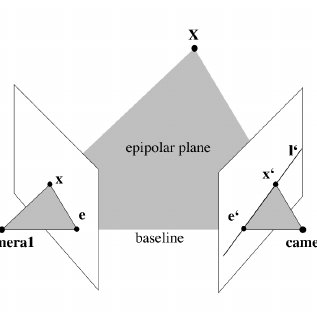
\includegraphics[width=0.6\textwidth]{epipolar2.jpg}
			\caption{Representação do plano epipolar.}
			\label{fig:esseciallinemat}
		\end{center}
	\end{figure}
	
	Sendo a matriz Essencial descrita desta forma, é possível obter os valores das matrizes rotação e translação através da decomposição dos valores singulares (\textbf{SVD}). Sendo : \[ E = U diag(1,1,0) V^{T} \] onde as duas soluções possíveis para a matriz rotação, R: \[ R = UWV^T \] \[ R = UW^TV^T \] e a matriz translação, t: \[ t = \pm u_3 \].
	
	
	Obtidas as matrizes rotação e translação existem 4 possíveis soluções, tal como verificado anteriormente. Desta forma, é necessário escolher a solução certa. Para testar as hipóteses é realizada a triangulação por regressão ortogonal e escolher a solução mais consistente.
	
	Desta forma, existe uma relação entre os pontos correspondentes entre imagens. Se um ponto desconhecido no mundo, \textbf{X}, representado na frame anterior como \textbf{x} e no frame atual como \textbf{x'}, as coordenas de \textbf{X} podem ser calculadas. Isto, requer a matriz intrinseca e a matriz Essencial entre frames.
	
	A relação entre os pontos da imagem, \textbf{x} e \textbf{x'} e o ponto no mundo \textbf{X} com os parâmetros da câmara P é expressa \[ x = P X \] \[ x' = P'X \], onde P e P' $\epsilon$  $\mathbb{R}^{3x4}$ é a combinação das matrizes intrinseca e Essencial do frame anterior e atual, respetivamente.
	
	Sendo, \[ x =  \left[ \begin{array}{ccc} u \\ v \\ 1 \end{array} \right],  x' =  \left[ \begin{array}{ccc} u' \\ v' \\ 1 \end{array} \right] ,  X =  \left[ \begin{array}{cccc} X_w \\ Y_w \\ Z_w \\ 1 \end{array} \right] \], \[ E =  \left[ \begin{array}{cccc} r_{11} & r_{12} & r_{13} & t_{x} \\ r_{21} & r_{22} & r_{23} & t_{y} \\ r_{31} & r_{32} & r_{33} & t_{z} \\ \end{array} \right] , K =  \left[ \begin{array}{ccc} f_x & 0 & x_c \\ 0 & f_y & y_c \\ 0 & 0 & 1 \\ \end{array} \right] \].
	
	Considerando $p^{iT}$ as linhas da matriz P e devido à estrutura da matriz instrinseca, K, X é expresso pela seguinte equação linear : \[ \left[ \begin{array}{cccc}
	up^{3T} - p^{1T} \\
	vp^{3T} - p^{2T} \\
	u'p'^{3T} - p'^{1T} \\
	v'p'^{3T} - p'^{2T} 
	\end{array} \right] X = 0 \].
	
	-resolver com SVD e obter um plano de features com as matchs
	-este plano é usado para calcular a média que limita  slow motion
	-obter coordenadas 2 deste plano. 
	-através de sen, cos (\textbf{descobrir como :o}) obtida a matriz R e translação correcta. 
	-concatenação da matriz
	-publicação.
	
	Devido aos movimentos curtos entre frames causaram maior erro, terem menor precisão no calculo do movimento, é necessário calcular a média do movimentos e aplicar um limite de forma a rejeitar movimentos curtos/lentos. Assim, o frame atual a analisar é rejeitado e analisamos um novo frame de forma a rejeitar movimentos curtos. 
	
	
	
	
	
	

\subsection{Desenvolvimento em Matlab}

O Matlab é um \textit{software} de alto desempenho desenvolvido para o cálculo numérico. Caracteriza-se por implementar uma linguagem própria que resulta de uma combinação de linguagens como C, Java e Basic.

O código desenvolvido em Matlab teve como função principal o processamento dos dados guardados nos \textit{rosbags}. Estes \textit{rosbags} contêm as mensagens publicadas para cada teste realizado. Foram desenvolvidos \textit{scripts} para filtrar os dados de interesse e gerar dados possíveis de analisar e inferir conclusões.

\section{Hardware}

Este subcapítulo visa apresentar os componentes de hardware utilizado no desenvolvimento do projeto.

\subsection{Raspberry Pi}

O Raspberry Pi é um computador do tamanho de um cartão de crédito.Todo o hardware é integrado numa única placa. O principal objetivo é promover o ensino em Ciência da Computação básica em escolas mas, devido à sua excelente qualidade / preço é bastante usado em grandes projetos de robótica, programação e até aplicações industriais. 

O modelo utilizado nesta dissertação é o Raspberry Pi 3 model B. Es modelo contem um processador 1.2 GHz 64-bit quad-core ARMv8 CPU, 1 GB de RAM e Bluetooth 4.1. Além disto, este computador é compatível com ROS Kinetic e com vários módulos , quais como a câmara com lente olho de peixe.

\begin{figure}[h!] %colocar figura a seguir ao texto anterior
	\begin{center}
		\leavevmode		
		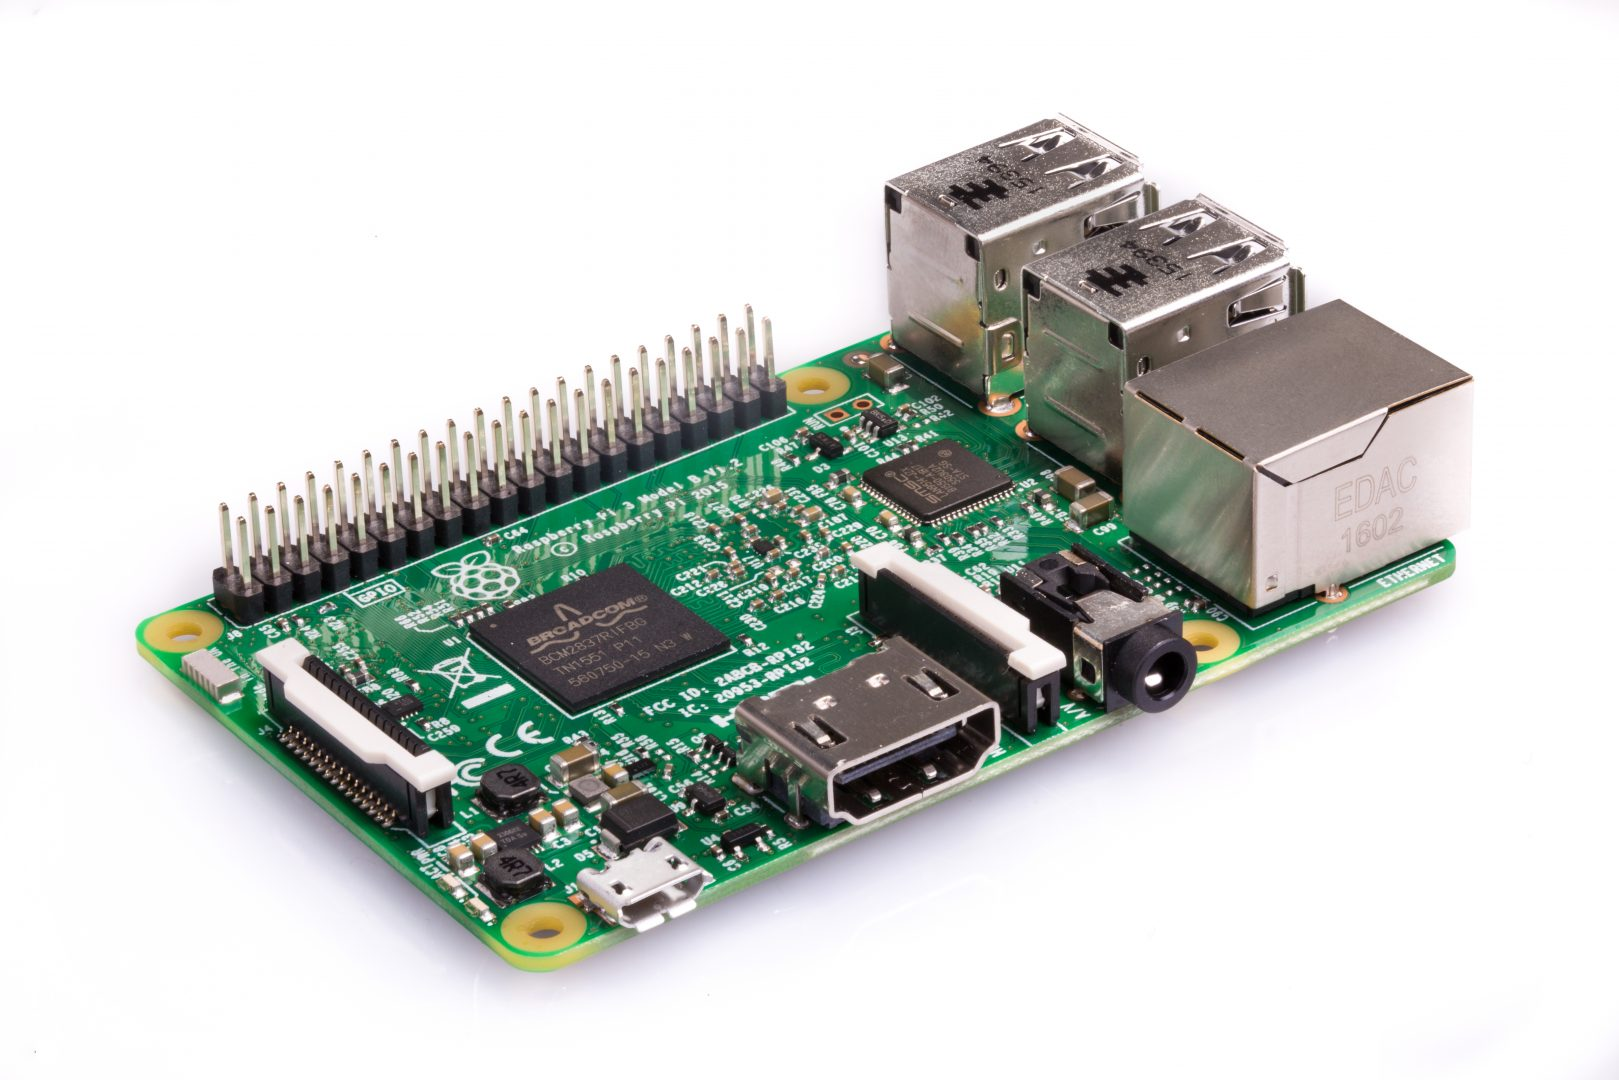
\includegraphics[width=0.6\textwidth]{raspberry.jpg}
		\caption{Exemplar da Raspberry Pi 3 modelo B.}
		\label{fig:raspberry}
	\end{center}
\end{figure}

\subsection{Câmara com lente olho de peixe}

A lente olho de peixe é uma lente grande angular que produz uma forte distorção visual destinada a criar uma imagem panorâmica ou hemisférica ampla. As lentes olho de peixe alcançam ângulos de visão extremamente amplos. Em vez de produzir imagens com linhas retas de perspetiva, as lentes olho de peixe usam um mapeamento especial (por exemplo: ângulo equissólido), que dá às imagens uma aparência convexa não retilínea.

\subsubsection{Tipos de lentes}

Existem 2 tipos de lentes olho de peixe, circular e \textit{full-frame}. 

Os primeiros tipos de lentes olho de peixe desenvolvidas foram circulares, lentes que tomaram um hemisfério de 180º projetando um circulo no plano de imagem. Estas, têm 180º de ângulo de visão vertical , horizontal e diagonal. 

As lentes olho de peixe \textit{full-frame} ampliam o círculo da imagem para cobrir toda a estrutura retangular, designado por "olho de peixe de moldura completa". Desta forma, as lentes têm um ângulo de visão diagonal de 180º enquanto os ângulos vertical e horizontal de visão são menores. 

A imagem ~\ref{fig:circularfullframe} representa as diferenças de plano de imagens obtidos com lente olhos de peixe circulares e olho de peixe \textit{full-frame} com ângulos de visão diagonal de 180º, 122º e 103,7º. 

Desta forma, como a aplicação da lente é no meio vinicula e num plano de imagem de uma lente olho de peixe circular maior parte da imagem é céu o uso da lente olho de peixe \textit{full-frame} é vantajoso para obter maior informação na horizontal do campo de visão e melhor na vertical.  

\begin{figure}[h!] %colocar figura a seguir ao texto anterior
	\begin{center}
		\leavevmode		
		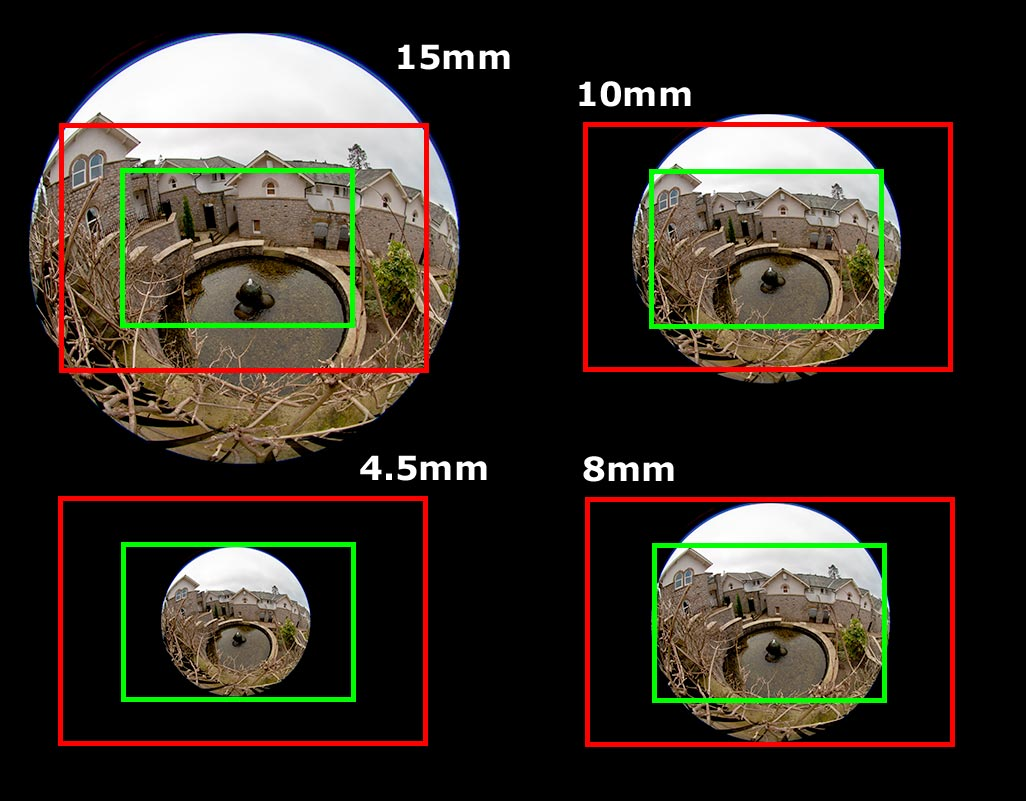
\includegraphics[width=0.6\textwidth]{circularfullframe.jpg}
		\caption{Diferença de ângulos de visão de lentes olho de peixe.}
		\label{fig:circularfullframe}
	\end{center}
\end{figure}


A lente especificamente escolhida é a representada na figura ~\ref{fig:lentfisheye}, com a seguintes especificações: 5 megapixel , angulo de abertura de 160 graus (câmaras têm tipicamente 72 graus), resolução 1080p e com suporte para LED infravermelho para visão noturna.

\begin{figure}[h!]%colocar figura a seguir ao texto anterior
	\begin{center}
		\leavevmode		
		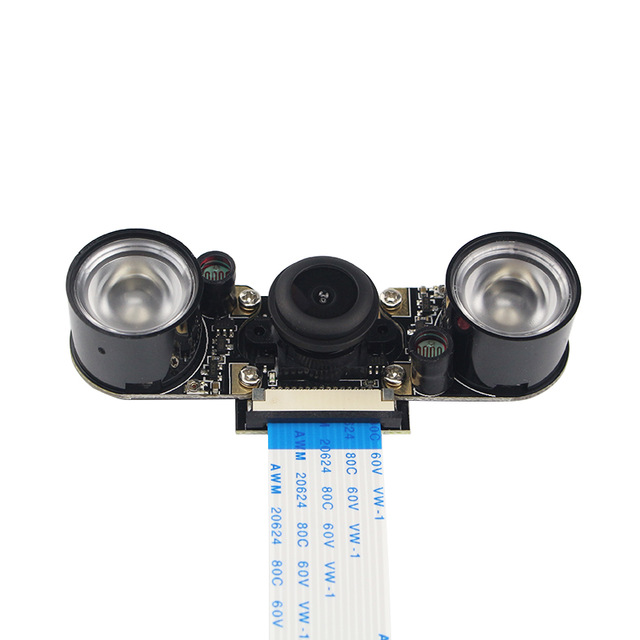
\includegraphics[width=0.4\textwidth]{lentfisheye}
		\caption{Câmara com lente olho de peixe e suporte para visão noturna.}
		\label{fig:lentfisheye}
	\end{center}
\end{figure}

	\chapter{Resultados Experimentais} \label{chap:resexp}


Os testes desta secção têm como objetivo encontrar o melhor detetor / descritor / matcher , determinando a robustez do subsistema de localização para o ruído, iluminação variante e rotação.

O detector de SURF possui um parâmetro personalizável, chamando minimo Hessian, que foi definido como 200. Esse valor foi recomendado por usuários que trabalham em aplicativos semelhantes e provaram trabalhar sob várias condições de brilho.

Para obter resultados repetíveis, a plataforma ROS permite ao usuário reproduzir uma sequência de mensagens nas mesmas condições em que foram adquiridas. Esta funcionalidade permite ao desenvolvedor resultados repetíveis, ou seja, diferentes combinações de parâmetros podem ser testadas para a mesma entrada exata.

\section{Testes}

De forma a validar o algoritmo de localização os testes requerem a quantificação do erro. O erro é descrito com a diferença entre o valor real e o valor medido.

As coordenadas reais têm de ser obtidas através de um sensor externo, tal como a laser baseado em loaclização, odometria das rodas or mesmo uma fita métrica. Devido ao declive dos terrenos e estrutura é utilizada uma fita métrica para comparação dos resultados.

Os devidos testes foram realizados em ambiente agricola, precisamente numa vinha. Os percursos efectuados foram : estático, movimento em linha reta, movimento em L (semi-quadrado), percurso quadrangular, percurso retangular e percurso circular. De notar que os percursos foram realizados com velocidades baixas. Assim, a câmara consegue extrair um maior número de caracteristicas e por consequência o erro da trajetória estimada será menor.  


\subsection{Teste de parâmetros}

Quatro parâmetros foram escolhidos para comparar a combinação dos detetores / descritores e matchers. Eles são :

\begin{itemize}
	\item \textbf{Imagens processadas} - Corresponde ao número de imagens que o programa conseguiu processar. É proporcional à velocidade do ciclo de processamento.
	\item \textbf{Média de frames perdidos} - Quantidade de frames perdidos entre ciclos.
	\item \textbf{Média matches por imagem} - Corresponde à média de correspondências encontradas para cada imagem depois de filtrar outliers.
	\item \textbf{Média de processamento} - Corresponde à média da duração de processamento de ciclo.
\end{itemize}


\subsection{Sequência sem Movimento}

Devido à fita métrica não produzir medidas em tempo real do movimento, o primeiro teste é feito com uma sequência de frames, or bags, onde o robô não se movimenta. Os testes foram realizados para 6 diferentes localizações com diferentes ambientes, iluminação e inclinações.

\subsection{Deteção da trajetória}

Devido ao erro deste teste não poder ser quantificado, este serve apenas como demonstração ou provas de conceito. A validação do resultado é visual.


	\chapter{Conclusões e Trabalho Futuro} \label{chap:conclF}

\section{Conclusões}

\section{Trabalho Futuro}

	%% Comment next 2 commands if numbered appendices are not used
	%\appendix
	%\chapter{Loren Ipsum} \label{ap1:loren}

Depois das conclusões e antes das referências bibliográficas,
apresenta-se neste anexo numerado o texto usado para preencher a
dissertação.

\section{O que é o \emph{Loren Ipsum}?}

\emph{\textbf{Lorem Ipsum}} is simply dummy text of the printing and
typesetting industry. Lorem Ipsum has been the industry's standard
dummy text ever since the 1500s, when an unknown printer took a galley
of type and scrambled it to make a type specimen book. It has survived
not only five centuries, but also the leap into electronic
typesetting, remaining essentially unchanged. It was popularised in
the 1960s with the release of Letraset sheets containing Lorem Ipsum
passages, and more recently with desktop publishing software like
Aldus PageMaker including versions of Lorem Ipsum~\citep{kn:Lip08}. 

\section{De onde Vem o Loren?}

Contrary to popular belief, Lorem Ipsum is not simply random text. It
has roots in a piece of classical Latin literature from 45 BC, making
it over 2000 years old. Richard McClintock, a Latin professor at
Hampden-Sydney College in Virginia, looked up one of the more obscure
Latin words, consectetur, from a Lorem Ipsum passage, and going
through the cites of the word in classical literature, discovered the
undoubtable source. Lorem Ipsum comes from sections 1.10.32 and
1.10.33 of ``de Finibus Bonorum et Malorum'' (The Extremes of Good and
Evil) by Cicero, written in 45 BC. This book is a treatise on the
theory of ethics, very popular during the Renaissance. The first line
of Lorem Ipsum, ``Lorem ipsum dolor sit amet\ldots'', comes from a line in
section 1.10.32.

The standard chunk of Lorem Ipsum used since the 1500s is reproduced
below for those interested. Sections 1.10.32 and 1.10.33 from ``de
Finibus Bonorum et Malorum'' by Cicero are also reproduced in their
exact original form, accompanied by English versions from the 1914
translation by H. Rackham.

\section{Porque se usa o Loren?}

It is a long established fact that a reader will be distracted by the
readable content of a page when looking at its layout. The point of
using Lorem Ipsum is that it has a more-or-less normal distribution of
letters, as opposed to using ``Content here, content here'', making it
look like readable English. Many desktop publishing packages and web
page editors now use Lorem Ipsum as their default model text, and a
search for ``lorem ipsum'' will uncover many web sites still in their
infancy. Various versions have evolved over the years, sometimes by
accident, sometimes on purpose (injected humour and the like). 

\section{Onde se Podem Encontrar Exemplos?}

There are many variations of passages of Lorem Ipsum available, but
the majority have suffered alteration in some form, by injected
humour, or randomised words which don't look even slightly
believable. If you are going to use a passage of Lorem Ipsum, you need
to be sure there isn't anything embarrassing hidden in the middle of
text. All the Lorem Ipsum generators on the Internet tend to repeat
predefined chunks as necessary, making this the first true generator
on the Internet. It uses a dictionary of over 200 Latin words,
combined with a handful of model sentence structures, to generate
Lorem Ipsum which looks reasonable. The generated Lorem Ipsum is
therefore always free from repetition, injected humour, or
non-characteristic words etc. 

	
	%%----------------------------------------
	%% Final materials
	%%----------------------------------------
	
	%% Bibliography
	%% Comment the next command if BibTeX file not used, 
	%% Assumes that bibliography is in ``myrefs.bib''
	%para referenciar sites \bibliographystyle{abbrvnat}
	
	\bibliographystyle{ieeetr}
	\bibliography{bib}
	
	%% Index
	%% Uncomment next command if index is required, 
	%% don't forget to run ``makeindex tese'' command
	%\PrintIndex
	
\end{document}
